\documentclass[a4paper,11pt]{report}

\usepackage[left=20mm,right=20mm,top=20mm,bottom=20mm]{geometry}
\renewcommand{\baselinestretch}{1.5}

\usepackage{fancyhdr}

\usepackage{titlesec}
\titleformat{\chapter}{\normalfont\LARGE\bf}{\thechapter}{16pt}{\LARGE\bf}
\titlespacing*{\chapter}{0pt}{0pt}{16pt}
\setcounter{secnumdepth}{4}
\bibliographystyle{unsrt}


  
\usepackage{graphicx}
 \graphicspath{{figures/}}
\usepackage{float}
\usepackage{subcaption}
\usepackage[font=small,skip=11pt]{caption}

 \usepackage{atbegshi}% http://ctan.org/pkg/atbegshi
\AtBeginDocument{\AtBeginShipoutNext{\AtBeginShipoutDiscard}}

\usepackage[labelfont={bf,it},textfont=it]{caption}

\usepackage[multiple]{footmisc}

\usepackage[hidelinks]{hyperref}

\usepackage{amsmath}
\usepackage{amsfonts}
\usepackage{amssymb}

\usepackage{tocloft} 
\usepackage{xfrac}
\usepackage{color}


\usepackage{algorithmicx}
\usepackage{algorithm}
\usepackage{algpseudocode}
\algnewcommand\algorithmicinput{\textbf{Input:}}
\algnewcommand\INPUT{\item[\algorithmicinput]}

\usepackage{enumitem}% http://ctan.org/pkg/enumitem

\usepackage{lscape}
\usepackage{xcolor}
\setlength\cftparskip{-6pt}

\DeclareMathOperator*{\argmax}{arg\,max}
\DeclareMathOperator*{\argmin}{arg\,min}
%\setlength{\abovedisplayskip}{0pt}
%\setlength{\belowdisplayskip}{0pt}

\title{\Huge{\textbf{Entropy Search for Bayesian Optimisation Based on Parabolic Approximation}}}
\author{
\includegraphics [width=0.4\textwidth]{Oxford}\\
        \scshape\Large University Of Oxford\\
        \vspace{5cm}
        \scshape MEng Engineering Science\\        
        \Large Author: Binxin Ru, St Edmund Hall \\
        \Large Supervisor: Prof. Michael Osborne
       }
\date{Trinity Term 2016}
	
\begin {document}

\maketitle

\renewcommand{\abstractname}{Acknowledgements}
\begin{abstract}
I would like to express my greatest gratitude to my supervisor, Prof. Michael Osborne, for the inspiration, guidance and encouragement. It was really an enriching journey for me to work under your supervision and thank you for motivating and enlightening me when I was confused or depressed by the experimental results. I would also like to thank several Ph.D candidates in the Machine Learning Research Group. First, I'm really grateful of Jack Fitzsimons who has provided me with highly informative and systematic supervision during my summer research project, enabling me to develop a much more solid foundation in the field of machine learning. Second, I would like to thank Mark McLeod and Favour Mandanji Nyikosa for helping me better understand Predictive Entropy Search and helping me tackle some technical issues in implementing the algorithms. Finally, I want to thank Gabriele Abbati for discussing entropy based methods with me and helping me install some C packages. 
\end{abstract}

\renewcommand{\abstractname}{Abstract}

\begin{abstract}
Bayesian optimisation is a powerful technique for optimising black-box functions that are expensive to evaluate\cite{brochu2010tutorial}.  A popular category of Bayesian optimisation techniques is based on information theory and recommends evaluation locations by maximising the information gain about the global minimiser of the objective function. Predictive Entropy Search (PES) is an important representative of information-based techniques and has demonstrated good empirical performance. However, PES requires many approximations to implement and face several drawbacks in its applications. We develop a novel information-based alternative, namely Entropy Search for Bayesian optimisation based on parabolic approximation (ESBOPA), that smartly approximates the unknown objective function in a parabolic form and represent the global minimum explicitly with a hyperparameter $\eta$. In comparison with PES, our technique faces less constraints on the choice of appropriate covariance functions for the Gaussian process prior, works in output space instead of input space as well as circumvents the need for sampling global minimiser in entropy computation. We demonstrate that ESBOPA performs as well as PES and other popular Bayesian optimisation techniques in several empirical tests.

\end{abstract}

\tableofcontents

%%%%%%%%%%%%%%%%%%%%%%%%%%%%%%%%%%%%%%%%%%%%%%%%%
%%%%%%%%%%%%%%  Literature review %%%%%%%%%%%%%%%%%%%%%%%%%
%%%%%%%%%%%%%%%%%%%%%%%%%%%%%%%%%%%%%%%%%%%%%%%%%
\chapter{Introduction}

Optimisation problems arise in numerous fields ranging from science and engineering to economics and management. Such problem can be  expressed in a mathematical form: 
	\begin{equation}
		\min_{\mathbf{x} \in \chi} f(\mathbf{x})
	\end{equation}
where  $\chi$ is the constrained domain of interest and $f(\mathbf{x})$ is the objective function. Usually we deal with classical optimisation problems in which the objective function is known together with its derivatives or the function is cheap to evaluate \cite{hennig2012entropy}. However, in many situations, we face another type of optimisation problems for which the above assumptions do not apply. For example, in the cases of clinical trials, financial investments or constructing a sensor network, it is very costly to draw a sample from the latent function underlying the real-world processes. Thus, efficient use of data available is very important. The objective functions in such type of problems are also non-convex in general and act like black boxes whose closed-form expressions and derivatives are unknown \cite{brochu2010tutorial}. Bayesian optimisation is a powerful tool to tackle such optimisation challenges. 
\\\\
A core step in Bayesian optimisation is to definite an acquisition function which uses the available observations effectively to recommend the next query location. There are many types of acquisition functions ranging from improvement-based measures, such as Probability of Improvement \cite{kushner1964new} and Expected Improvement \cite{jones1998efficient}, to optimistic measures, such as Gaussian Process Upper Confidence Bound \cite{srinivas2009gaussian}. The most recent type, which is based on information theory, offers a brand new perspective to efficiently select the sequence of sampling locations based on entropy of the distribution over the unknown minimiser $\mathbf{x}_*$ \cite{shahriari2016taking}. The information-based approaches guide our evaluations to locations where we can maximise our learning about the unknown minimum rather than to locations where we expect to obtain lower functional values\cite{hennig2012entropy}. However, the existing information-based acquisition functions, mainly Entropy Search and Predictive Entropy Search, require many approximations to implement and face serious constraints in its application. This project aims to develop a novel information-based approach which has extended applicability and is much easier to implement. Specifically, our approach has three major advantages over the state-of-the-art technique (i.e. Predictive Entropy Search). First, our approach faces less constraints on the choice of appropriate covariance functions for the Gaussian process prior. Second, our approach focuses on the information content in output space instead of input space, thus more efficient in high dimensional problems. Third, our approach circumvents the need to generate minimiser samples for entropy computation, thus saving much efforts for the sampling process. Because of its reliance on the smart use of the parabolic expression, our novel acquisition function is called entropy search for Bayesian optimisation based on parabolic approximation (ESBOPA). 
\\\\
This report is organised into  three parts. To begin with, Chapter 2 provides a literature review on the relevant knowledge about Bayesian optimisation. The review covers the choice of the prior distribution for Bayesian optimisation and a general overview of several popular types of acquisition functions. Particularly, Predictive Entropy Search is discussed in detail because it is the state-of-the-art entropy-based approach. Chapter 3 focuses on the technical details of our ESBOPA approach. It starts with the core idea of approximating any objective function with a parabolic form to directly represent the global minimum as a hyperparameter $\eta$ and the use of local linearisation to make the approximation analysis tractable. The second section of the chapter goes through the derivation of ESBOPA approach as well as the methods adopted to compute various components of  ESBOPA acquisition function for implementation. This is followed by a discussion on the possible ways to treat hyperparameters in our inference. Finally, the series of experiments we used to test ESBOPA approach are explained in Chapter 4 and the performance of ESBOPA is compared with those of EI and PI.  
\\\\
%This report is organised into  three parts. To begin with, Chapter 2 provides a literature review on the relevant knowledge about Bayesian optimisation. The first key component of Bayesian optimisation is the prior distribution chosen to model the unknown objective function. The Gaussian process model, which is a popular choice for the prior and is adopted by our project, is introduced. The second key component is the acquisition function. We gives a brief overview of various types of acquisition functions ranging from improvement-based ones to the more recent information-based ones. Particularly, Predictive Entropy Search is discussed in detail because it is the state-of-the-art entropy-based approach.   %

\chapter{Literature Review}

% Section 1: Bayesian optimisation intro

\section{Bayesian Optimisation}
Bayesian optimisation is a power tool for finding the optimum of a black-box objective function which is costly to evaluate. It is particularly useful in the cases when the function does not have an analytical form but noisy observations of the function at sampled points can be obtained \cite{brochu2010tutorial}.  
\\\\
To perform Bayesian optimisation, we first decide a prior belief over the unknown objective functions and then update this prior model by incorporating observation data to obtain a Bayesian posterior. The posterior reflects our updated beliefs about the objective function based on data observed, . In order to take the next sample efficiently, we compute an acquisition function which harnesses the mean and variance of the posterior distribution to evaluate the utility of potential locations for the next evaluation. The next query location is then determined by maximising the acquisition function \cite{shahriari2016taking}. The procedures of Bayesian optimisation is summarised in Algorithm \ref{BO} \cite{brochu2010tutorial}. And Figure \ref{BOdemonstration} demonstrates three iterations of Bayesian optimisation on a 1D objective function. 
\\
% B.O. Algorithm 
\begin{algorithm}
\caption{Bayesian optimisation }\label{BO}
\begin{algorithmic}[1]
\Statex
	\For{n=1,$\dots $}
	\State select new $\mathbf{x}_{n+1}$ by optimising acquisition function $\alpha$ :   $\mathbf{x}_{n+1}=\argmax_{\mathbf{x}} \alpha(\mathbf{x} \vert D_n ) $
	\State evaluate the objective function to obtain $y_{n+1}$
	\State augment observation data $D_{n+1} = \{ D_n, (\mathbf{x}_{n+1} , y_{n+1}) \} $
	\State update statistical model 
	\EndFor
\end{algorithmic}
\end{algorithm}
\\
\noindent
In essence, Bayesian optimisation approach has two key components: 1) the prior distribution that represents our belief on the unknown objective function and 2) the acquisition function that evaluates the utility of possible query points and recommend the next point that would lead to utility maximisation.   
\\
\begin{figure} [H]
	\label{BOdemonstration}
	\centering
	 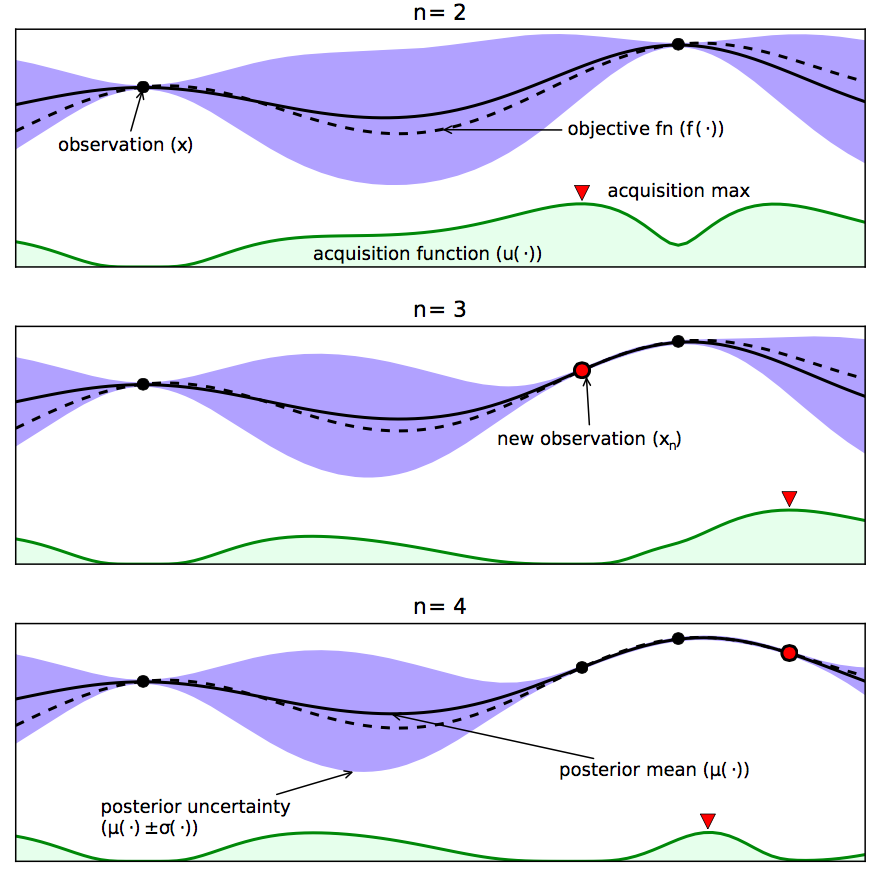
\includegraphics[width=0.7\linewidth]{Bayesianoptimisation.png}
\caption{ Demonstration of the use of Bayesian optimisation on a 1D example. The figure shows  the mean and confidence intervals of the Gaussian process model that approximates the objective function. The acquisition function (green) is high where the Gaussian process model predicts a high objective (exploitation) and where the prediction uncertainty is high (exploration). It is interesting to note that the region on the far left remains unsampled because while it has high uncertainty, it is correctly predicted to offer little improvement over the highest observation \cite{brochu2010tutorial}  }
\end{figure}

\subsection{The Gaussian Process Prior}
Bayesian optimisation requires the definition of a prior distribution. When the number of observation is large, a prior distribution can enable convergence to the global optimum of the objective function if 1) the acquisition function is continuous and  approximately minimises the expected deviation from the global minimum at a query point  and 2) the conditional variance converges to zero at the observation data \cite{mockus1994application}.  Many prior models fulfil these conditions but in this project, we choose to use the Gaussian process which is a popular non-parametric model.
\\\\
The Gaussian process is a collection of random variables, any finite number of which have a multivariate Gaussian distribution \cite{rasmussen2006gaussian}. It is fully specified by a mean function $m$ and 
a covariance function $k$ \cite{rasmussen2006gaussian}: 
	\begin{equation}
	f(\mathbf{x}) \sim \mathcal{GP} \big( m(\mathbf{x}),k(\mathbf{x},\mathbf{x}')\big).
	\end{equation}
\noindent	
At an arbitrary input $\mathbf{x} $, a Gaussian process returns the mean and variance of a normal distribution over the possible values of  $f(\mathbf{x}) $ \cite{brochu2010tutorial}. The mean function of the prior distribution provides an offset and specifies our inference far from observations \cite{C24 Advanced probability notes}. For simplicity, the mean function is usually set to zero \cite{rasmussen2006gaussian} and thus, the Gaussian process prior is solely determined by the covariance function.
\\\\
By sampling the objective function at $n$ input locations, we obtain observation data $D_{f}=\{(\mathbf{x}_i,f_i) \vert i = 1, \dots, n \}=\{(\mathbf{X}_n,\mathbf{f}_n)\}$.  The function values  $\mathbf{f}_n$ are drawn based on the multivariate normal distribution $p(\mathbf{f}_n)= \mathcal{N}\big( \mathbf{f}_n; \mathbf{0},K( \mathbf{X}_n,\mathbf{X}_n) \big)$, where each element of the covariance matrix $K$ is defined as $K_{ij}=k(\mathbf{x}_i,\mathbf{x}_j)$.
\\\\
The joint distribution of the observed function values $\mathbf{f}_n$ and the function value at a test location $ f=f(\mathbf{x}) $ is also Gaussian \cite{rasmussen2006gaussian} :
\begin{equation}
	\begin{bmatrix}
  		 \mathbf{f}_n\\ 
   		f
	  \end{bmatrix}
		\sim\mathcal{N} \left ( 
 		\begin{bmatrix}
   		K(\mathbf{X}_n,\mathbf{X}_n) & K(\mathbf{X}_n,\mathbf{x}) \\
   		K( \mathbf{x}, \mathbf{X}_n) & K( \mathbf{x}, \mathbf{x})
 	\end{bmatrix} \right ).
 \end{equation} 
By manipulating the joint distribution, we obtain the predictive posterior distribution at the test point $\mathbf{x}$:
\begin{equation} \label{posteriorf}
	p(f \vert \mathbf{x},\mathbf{X}_n, \mathbf{f}_n) = \mathcal{N}\big( f ; m_{f}(\cdot), K_{f}(\cdot, \cdot) \big)
\end{equation}
where 
\begin{equation} 
	m_{f}(\mathbf{x})=K(\mathbf{x}, \mathbf{X}_n) K(\mathbf{X}_n,\mathbf{X}_n)^{-1} \mathbf{f}_n 
\end{equation}
\begin{equation} \label{covarianceofposter}
	K_{f}(\mathbf{x},\mathbf{x}')=  K(\mathbf{x},\mathbf{x}') - K( \mathbf{x},\mathbf{X}_n ) K(\mathbf{X}_n,\mathbf{X}_n)^{-1} K(\mathbf{X}_n,\mathbf{x}).
\end{equation} 
\\
However, in real word situation, we do not have access to the true function values but only noisy observation of the function $ y(\mathbf{x}_i) = f(\mathbf{x}_i) +  \epsilon $ where $\epsilon$ is assumed to be an independently and identically distributed Gaussian noise with variance $\sigma_n^2$ \big(i.e. $p(\mathbf{y} \vert \mathbf{f}) = \mathcal{N} ( \mathbf{f}, \sigma_n^2 \mathbf{I}) \big)$ \cite{rasmussen2006gaussian}.  In the case of noisy observation data $D_n=\{(\mathbf{x_{i}},y_{i}) \vert i=1, \dots n\}=\{ \mathbf{X}_n,\mathbf{y}_n\}$, the Gaussian process prior becomes $p (\mathbf{y}_n)= \mathcal{N}\big(\mathbf{y}_n; \mathbf{0},K( \mathbf{X}_n,\mathbf{X}_n)+\sigma_n^2 \mathbf{I} \big)$. The predictive distribution of the noisy observation $y$ at the test point $\mathbf{x}$ has the form
 	\begin{equation} \label{posteriory}
	p(y \vert \mathbf{x},\mathbf{X}_n, \mathbf{f}_n) =\mathcal{N} \big( y ; m_{y}(\cdot), K_{y}(\cdot, \cdot) \big)
 	\end{equation}
where 
\begin{equation} 
	m_{y}(\mathbf{x})=K(\mathbf{x}, \mathbf{X}_n) \big[ K(\mathbf{X}_n,\mathbf{X}_n) +\sigma_n^2 \mathbf{I} \big]^{-1} \mathbf{y}_n 
\end{equation}
\begin{equation} 
	K_{y}(\mathbf{x},\mathbf{x}')=  K(\mathbf{x},\mathbf{x}') - K(\mathbf{x}, \mathbf{X}_n)\big[ K(\mathbf{X}_n,\mathbf{X}_n)+\sigma_n^2 \mathbf{I} \big]^{-1} K(\mathbf{X}_n,\mathbf{x}).
\end{equation}

%% %%
\subsubsection{Covariance Functions}
The choice of covariance function is essential for a Gaussian process because it affects the smoothness properties of the Gaussian process prior \cite{brochu2010tutorial} and thus determines the structure of the response functions we can model \cite{shahriari2016taking}. A covariance function is valid if its Gram matrix $K$ whose element is $K_{ij}=k(\mathbf{x}_i,\mathbf{x}_j)$ is positive semidefinite and valid covariance functions can be expressed as an inner product  in the feature space $k(\mathbf{x}_i,\mathbf{x}_j)=\phi(\mathbf{x}_i)^T\phi(\mathbf{x}_j)$ \cite{bishop2006pattern}. New valid covariance functions can be efficiently constructed by manipulating proven simple covariance functions (e.g. multiplying and/or adding simple covariances) \cite{rasmussen2006gaussian}. 
\\\\
In this project, we use the squared exponential covariance function with automatic relevance determination  (SE-ARD), which is a popular type of covariance functions that allows us to learn the characteristic length scales in each input dimension. Characteristic length scales measure the distance we need to move in input space for the function values to be uncorrelated \cite{rasmussen2006gaussian}. If the characteristic length scale of a certain input is very large,  the covariance will become almost independent of that input as shown in Figure \ref{seard}.
\\\\
The analytical form of the squared exponential ARD covariance function is 
\begin{equation}
 k(\mathbf{x}_i,\mathbf{x}_j)=\sigma^2 \exp \left[-\frac{1}{2}(\mathbf{x}_i-\mathbf{x}_j)^T \Lambda_l^{-2} (\mathbf{x}_i-\mathbf{x}_j) \right]
 \end{equation}
where $\sigma$ is the output scale  and $\Lambda_l$ is a diagonal matrix of $D$ length scales. 
\\
\begin{figure} [H]
	\label{seard}
	\centering
	 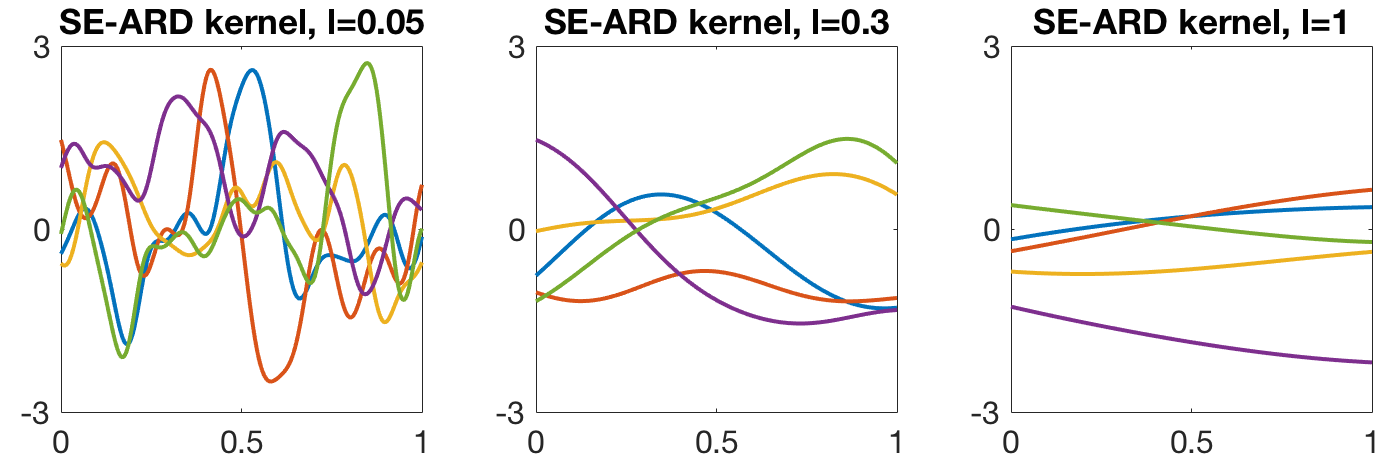
\includegraphics[width=0.8\linewidth]{SEARDprior.png}
\caption{ Random samples generated by a Gaussian process prior with the SE-ARD covariance function and different characteristic lengths.}
\end{figure}
\noindent 

\newpage
%% Acquisition functions  %%
\subsection{Acquisition Functions } \label{acqusitionfunction}

Acquisition functions are carefully designed to balance exploration and exploitation. Thus, they would recommend the next query location where the function value predicted by the posterior distribution is high (exploitation ) and/or the uncertainty is large (exploration) \cite{brochu2010tutorial}. As compared to the objective function, the acquisition functions must be much cheaper to evaluate or approximate and thus can be optimised more easily \cite{shahriari2016taking}. In this section, we would introduce three main categories of acquisition functions: 1) improvement-based acquisition functions, 2) optimistic acquisition functions and 3) the information-based acquisition functions.

\subsubsection{Improvement-based Acquisition Functions}

\textbf{{Probability of Improvement}}
\\\\
An simple form of acquisition function developed early in 1964 is Probability of Improvement (PI) \cite{kushner1964new}. PI method measures the probability that a location $\mathbf{x}$ leads to an improvement upon the incumbent maximum value observed  $f(\mathbf{\hat{x}})$ where $\mathbf{\hat{x}}=\argmax_{\mathbf{x}_{i}} f(\mathbf{x}_{i})$ for $i=1, \dots, n$. This probability is computed in the form of a cumulative distribution function\cite{brochu2010tutorial}: 
	\begin{equation}
	\alpha_{PI}(\mathbf{x} \vert D_n) = Prob(f(\mathbf{x})\geq f(\mathbf{\hat{x}}))=\Phi \left (\dfrac{ m (\mathbf{x})-f(\mathbf{\hat{x}})}{\sigma(\mathbf{x})} \right) 
	\end{equation}
where $\Phi$ is the standard normal cumulative distribution and $m (\mathbf{x}) $ and $\sigma(\mathbf{x})$ are the mean and standard deviation of the posterior distribution at a test location $\mathbf{x}$. The next sample is then taken at the location with the maximum $\alpha_{PI}(\mathbf{x} \vert D_n) $ .
\\\\
PI acquisition function tends to be highly exploitation-oriented. To encourage more exploration, Kushner \cite{kushner1964new} proposes to add a positive trade-off parameter $\zeta $ so that PI method would recommend the next point by maximising the probability of improving over $f(\mathbf{\hat{x}})+ \zeta$. However, the value of $\zeta$ is often set arbitrarily. If $\zeta$ is too small, the search will be highly local whereas if $\zeta$ is too high, the search will be global but slow to converge \cite{jones2001taxonomy}.
\\\\	
\textbf{Expected Improvement}
\\\\
Expected Improvement (EI) acquisition function offers an alternative to PI method by considering the magnitude of improvement\cite{dixon1978towards} \cite{jones1998efficient}. In EI acquisition function, the utility is represented by an improvement function $I(\mathbf{x})$ which is defined as

\begin{equation}
	I(\mathbf{x})=max\{ 0, f(\mathbf{x})-f(\mathbf{\hat{x}})\}.
\end{equation}
$ I(\mathbf{x}) $ is positive only when the prediction at the test location leads to an improvement over the maximum value known thus far $f(\mathbf{\hat{x}})$. Otherwise, $ I(\mathbf{x}) $ is zero. The new query point is then recommended by maximising the expected improvement 
   	\begin{equation}
	\mathbf{x}=\argmax_\mathbf{x} \mathbb{E} [ I(\mathbf{x}) \vert D_n  ].
	\end{equation}
The expectation can be computed analytically \cite{dixon1978towards}:
\begin{eqnarray*} 
\alpha_{EI}(\mathbf{x} \vert D_n) &= & \mathbb{E} [ I(\mathbf{x}) \vert D_n  ]
	\\ &=& \int\limits_{0}^{\infty} I(\mathbf{x}) \mathcal{N} \big(I; m (\mathbf{x})-f(\mathbf{\hat{x}}), \sigma(\mathbf{x})^2 \big) \mathrm{d} I(\mathbf{x}) 
	\\ & = & 
\begin{cases}
	\big(m({\mathbf{x}})-f(\mathbf{\hat{x}})\big) \Phi \left( \dfrac {m(\mathbf{x})-f(\mathbf{\hat{x}})}{\sigma({\mathbf{x}})} \right) + \sigma(\mathbf{x}) \phi \left( \dfrac {m(\mathbf{x})-f(\mathbf{\hat{x}})}{\sigma({\mathbf{x}})} \right) & \text{if}  \hspace{11pt} \sigma(\mathbf{x}) > 0 \\
	0				    & \text{if} \hspace{11pt}  \sigma(\mathbf{x}) = 0
\end{cases}	
\end{eqnarray*}
\noindent
where $\Phi$ and  $\phi$ denotes the cdf and pdf of the standard normal distribution, and $m(\mathbf{x})$ and $\sigma(\mathbf{x})$ are the mean and standard deviation of the posterior distribution at a test location $\mathbf{x}$. 
\\\\
The two terms in EI acquisition function balances the trade-off between exploitation and exploration respectively. Similar to the PI case, Lizotte \cite{lizotte2008practical}  proposes to incorporate a parameter $\zeta$ into EI acquisition function to control the trade-off between local optimisation and global search. Lizotte's experiments suggeste that $\zeta=0.01$ works well in almost all cases. 

\subsubsection{Optimistic Acquisition Functions}

\textbf{Upper Confidence Bound}
\\\\
The concept of using confidence bounds for Bayesian optimisation is first explored by Cox and John \cite{cox1992statistical} in their Sequential Design for Optimisation(SDO) algorithm. SDO recommends the next point for evaluation by maximising the following acquisition function: 
\begin{equation} \label{upc}
	\alpha_{UCB}(\mathbf{x} \vert D_n) = m(\mathbf{x}) + \kappa \sigma(\mathbf{x}).
\end{equation} 
which is a weighted sum of posterior mean $m(\mathbf{x})$ and standard deviation $\sigma(\mathbf{x})$, thus incorporating the trade-off between exploitation and exploration. $\kappa$ is a parameter set by the user.
\\\\
Srinivas et al. \cite{srinivas2009gaussian} then propose a guideline for setting and scheduling the value of $\kappa$ which can lead to minimisation of the cumulative regret:  
\begin{equation}
	R_{n} = \sum_{i=1}^n f(\mathbf{x}_{*}) - f(\mathbf{x}_{i})
\end{equation}
where $\mathbf{x}_{*} $ is the true global maximiser and $\mathbf{x}_i$ is the query point selected via the acquisition function. With this guideline, they define the Gaussian Process Upper Confidence Bound (GP-UCB) whose acquisition function is a modified version of Equation \ref{upc}: 
\begin{equation} \label{gp-upc}
	\alpha_{GP-UCB}(\mathbf{x} \vert D_n) = m(\mathbf{x}) + \sqrt{\upsilon \tau_{n}} \sigma(\mathbf{x})
\end{equation} 
where $\upsilon>0$ and $\tau_n=2 \log(n^{d/2+2}\pi^2 / 3\delta)$. $d$ is the input dimension and $n$ is the number of observation taken.
%%
\subsubsection{Information-based Acquisition Function} \label{Infoaf}

\textbf{Entropy Search}
\\\\
Entropy Search (ES) \cite{hennig2012entropy} aims to reduce the uncertainty about the unknown global minimiser $\mathbf{x}_*$ by selecting a query point that leads to the largest reduction in entropy of the distribution $p(\mathbf{x}_* \vert D_n)$. The acquisition function for ES has the form \cite{hennig2012entropy}: 
\begin{equation} \label{ESacuqisitionfunction}
	\alpha_{ES} (\mathbf{x} \vert D_n )=H[p(\mathbf{x}_{*} \vert D_n)]-\mathbb{E} _{p(y \vert D_n,\mathbf{x})} \Big[H \big[p \big( \mathbf{x}_{*} \vert D_n \cup {(\mathbf{x},y)} \big) \big] \Big] 
\end{equation}
where $H[p(\mathbf{x})] = - \int p(\mathbf{x}) \log p(\mathbf{x}) \mathrm{d} \mathbf{x} $ and the expectation is taken with respect to the posterior distribution $p(y \vert D_n,\mathbf{x}) $. 
\\\\
The first differential entropy term in the above function embodies our current uncertainty about the unknown minimiser $\mathbf{x}_*$. The second term measures our expected uncertainty about $\mathbf{x}_*$ after querying an arbitrary point $(\mathbf{x},y)$. Thus, the acquisition function (Equation \ref{ESacuqisitionfunction}), which is the difference between the two entropy terms, represents the information gain about  $\mathbf{x}_*$ and ES method would select the point that maximise this information gain.
\\\\
However, an exact evaluation of the ES acquisition function (Equation \ref{ESacuqisitionfunction}) is only feasible after many approximations because the entropy terms cannot be computed analytically and the optimisation of Equation \ref{ESacuqisitionfunction} involves calculating $p \big(\mathbf{x}_{*} \vert D_n \cup {(\mathbf{x},y)} \big)$ for many different values of $\mathbf{x}$ and $y$ \cite{hernandez2014predictive}. The approximation proposed by \cite{hennig2012entropy} is based on discretisation of the continuous search space, which results in a high computational costs of $O(M^4)$ where $ M $ is the number of discrete representer points. 
\\\\
\textbf{Predictive Entropy Search}
\\\\
In view of the difficulties of implementing ES method, Lobato et al.\cite{hernandez2014predictive} propose a modified alternative,  named Predictive Entropy Search(PES). PES method utilises the symmetric property of mutual information and rewrite Equation \ref{ESacuqisitionfunction} as \cite{hernandez2014predictive} : 
\begin{equation} \label{PESacqfunc}
\alpha_{PES} (\mathbf{x} \vert D_n )=H[p(y \vert D_n,\mathbf{x})]-\mathbb{E} _{p(\mathbf{x}_{*} \vert D_n)}[H[p(y \vert D_n,\mathbf{x},\mathbf{x}_{*})]]
\end{equation}
where $p(y \vert D_n,\mathbf{x},\mathbf{x}_{*})$ is the posterior distribution for $y$ conditioned on the observation data $D_n$, the test point $\mathbf{x}$ and the global maximiser $\mathbf{x}_{*}$. Different from ES acquisition function(Equation \ref{ESacuqisitionfunction}) which depends on the entropies of distributions on maximiser $\mathbf{x}_{*}$, the PES acquisition function (Equation \ref{PESacqfunc}) uses the entropies of predictive posterior distributions over output $y$ which can be computed analytically or be approximated more easily \cite{hernandez2014predictive}.
\\\\
PES has been shown to achieve better optimisation performance than ES  while requiring  less computational costs to be implemented. Thus, PES is the state of the art in information-based approaches. We will discuss PES method in more details in Section \ref{PESsection} because our project takes PES as a basis and develops a novel information-based approach, named Entropy Search for Bayesian optimisation based on quadratic approximation (ESBOPA).

\subsection{Predictive Entropy Search} \label{PESsection}
\subsubsection{Algorithm} \label{PESderivation}

As mentioned above, the acquisition function for PES has the form: 
\begin{equation} \label{PESacqfunc2}
\alpha_{PES} (\mathbf{x} \vert D_n )=H[p(y \vert D_n,\mathbf{x})]-\mathbb{E} _{p(\mathbf{x}_{*} \vert D_n)}[H[p(y \vert D_n,\mathbf{x},\mathbf{x}_{*})]].
\end{equation}
The first entropy term in Equation \ref{PESacqfunc2} has closed-form as the posterior distribution is a Gaussian:  
\begin{equation}
 H[p(y \vert D_n,\mathbf{x})] = 0.5 \log [2 \pi e ( v_n (\mathbf{x}) + \sigma_n^2)]
 \end{equation}
 where $v_n (\mathbf{x})$ is the variance of the posterior distribution at a test point $\mathbf{x}$ which can be computed using Equation \ref{covarianceofposter} and $\sigma_n^2$ is the variance of observation noise.  The second term cannot be computed analytically and we need sophisticated techniques to approximate the expectation, the predictive posterior distribution $p(y \vert D_n,\mathbf{x},\mathbf{x}_{*})$ as well as the entropy of this distribution \cite{hernandez2014predictive}. 
\\\\
First, the expectation can be approximated by drawing Thompson samples of maximisers $\mathbf{x}_{*} $ from $p(\mathbf{x}_{*} \vert D_n)$ and then compute the average entropy over all samples \cite{hernandez2014predictive}. According to Bochner's theorem \cite{bochner2016lectures}, any continuous stationary covariance function $k$ has a corresponding spectral density $s(\mathbf{w})$ obtained by Fourier transform. Using the normalised version of the spectral density $p(\mathbf{w})=s(\mathbf{w}) /\alpha$, the covariance function can be re-expressed as 
\begin{equation}
	k(\mathbf{x},\mathbf{x}') = \alpha \mathbb{E}_{p(\mathbf{w})} \left[ \exp [ - i \mathbf{w}^ {T} (\mathbf{x} - \mathbf{x}') ] \right] = 2 \alpha \mathbb{E}_{p(\mathbf{w}, b)} \left[ \cos(\mathbf{w}^ {T} \mathbf{x} + b) \cos(\mathbf{w}^ {T} \mathbf{x}' + b) \right]
\end{equation}
\noindent where $ b \sim \mathcal{U} [0, 2 \pi] $ \cite{rahimi2007random}. By using an $m$-dimensional feature vector $\phi(\mathbf{x}) = \sqrt{2 \alpha /m } \cos(\mathbf{W} \mathbf{x} + \mathbf{b})$ where $\mathbf{W} $ and $\mathbf{b} $ are $m$ stacked samples from $p(\mathbf{w},b)$, we can rewrite the covariance function as $ k(\mathbf{x},\mathbf{x}')  \approx \phi(\mathbf{x}) ^T  \phi(\mathbf{x}') $ and approximate the prior for the objective function with a linear model $ f(\mathbf{x}) = \phi(\mathbf{x}) ^T \boldsymbol{\psi} $\cite{hernandez2014predictive}. $\boldsymbol{\psi} $ is a standard multivariate Gaussian whose posterior distribution is also a Gaussian:
	 \[ \boldsymbol{\psi} \sim \mathcal{N} ( \mathbf{0}, \mathbf{I})  \hspace{12pt} \text{and}  \hspace{12pt}  \boldsymbol{\psi} \vert D_n \sim \mathcal{N} \left( (\boldsymbol{\Phi}^T \boldsymbol{\Phi} + \sigma_n^2 \mathbf{I})^{-1} \boldsymbol{\Phi}^T \mathbf{y}_n,   \sigma_n^2 (\boldsymbol{\Phi}^T \boldsymbol{\Phi} + \sigma_n^2 \mathbf{I})^{-1} \right) \]	
where $\boldsymbol{\Phi}^T = [ \boldsymbol{\phi} (\mathbf{x}_1) \dots \boldsymbol{\phi} (\mathbf{x}_n) ] $ \cite{hernandez2014predictive}. Now we can sample the maximiser $\mathbf{x}_{*}^{(i)}$ by minimising the approximated posterior sample of $f^{(i)}$: 
\begin{equation}
\mathbf{x}_{*}^{(i)}= \argmin_\mathbf{x} f ^{(i)}(\mathbf{x}) =  \argmin_\mathbf{x} \phi^{(i)} (\mathbf{x}) ^{T} \boldsymbol{\psi} ^{(i)}.
\end{equation}
\\
Another key component of PES acquisition function is the  predictive posterior distribution which can be computed via marginalisation: $p(y \vert D_n,\mathbf{x},\mathbf{x}_{*}) = \int p \big(y \vert f(\mathbf{x}) \big) p \big( f(\mathbf{x}) \vert D_n, \mathbf{x}, \mathbf{x}_{*} \big) \mathrm{d} f(\mathbf{x})$. The likelihood function is a Gaussian $ p\big(y \vert f(\mathbf{x}) \big) = \mathcal{N} \big(y ; f(\mathbf{x}), \sigma_n^2 \big) $. The posterior distribution $p \big( f(\mathbf{x}) \vert D_n, \mathbf{x}, \mathbf{x}_{*} \big) $ is intractable because it is conditioned on the global maximiser $\mathbf{x}_{*}$.  Lobato et al.\cite{hernandez2014predictive} overcome this intractability by using three simplified constraints (C1,C2,C3) and approximate the posterior distribution in the form: $p ( f(\mathbf{x}) \vert D, \mathbf{x}, \mathbf{x}_{*}) = p ( f(\mathbf{x}) \vert D, C1,C2,C3) $. 
\\\\
The three constraints are as follows:
\\
\textbf{C1. $\mathbf{x}_{*}$ is a local maximiser.} This is satisfied if $\bigtriangledown f(\mathbf{x}_{*}) = \mathbf{0}$ (C 1.1) and $\bigtriangledown^2 f(\mathbf{x}_{*}) $ is negative definite (C 1.2).  Lobato et al.\cite{hernandez2014predictive} further simplify (C 1.2) by assuming that the non-diagonal elements of $\bigtriangledown^2 f(\mathbf{x}_{*}) $, denoted as  upper $[\bigtriangledown^2 f(\mathbf{x}_{*}) ]] $, are zeros. Thus, the constraint C 1.2 becomes that the diagonal elements of the Hessian matrix $[\bigtriangledown^2 f(\mathbf{x}_{*})]$ are negative. 
\\
\textbf{C2. $f(\mathbf{x}_{*})$ is larger than current observations.} This implies $f(\mathbf{x}_{*}) \geq f(\mathbf{x}_{i})$ for $i \leq n$. However, in reality, we only have noisy observations $y_i$. To avoid performing inference on the true function values, the above inequality is approximated with a looser constraint $f(\mathbf{x}_{*}) > y_{max} + \epsilon $ where $ \epsilon$ is a zero-mean Gaussian noise with variance $\sigma_{n}^{2}$ and $y_{max}$ is the largest observation. 
\\
\textbf{C3. $ f(\mathbf{x}_{*})$  is greater than $f(\mathbf{x}). $}  This constraint means that we will consider the test point location $\mathbf{x} $ only if $f(\mathbf{x}_{*}) \geq f(\mathbf{x})$. 
\\\\
The three constraints are incorporated into $p ( f(\mathbf{x}) \vert D_n)$ by multiplying it with factors that embodies these constraints. The approximation procedures are described briefly below and more detailed derivations can be found in \cite{hernandez2014predictive}.  
\\\\
First, Lobato et al. define two random variables $\mathbf{c} = \big[ \mathbf{y}_n ; \bigtriangledown f(\mathbf{x}_{*}) ; \text{upper} [\bigtriangledown^2 f(\mathbf{x}_{*}) ] \big] = [ \mathbf{y}_n; \mathbf{0};  \mathbf{0}] $ and $\mathbf{z} = \big[ f(\mathbf{x}_*) ; \text{diag} [\bigtriangledown^2 f(\mathbf{x}_{*})] \big]$. The constraint C 1.1 is enforced by conditioning on $\mathbf{c}$:
\begin{equation} \label{C11}
	p( \mathbf{z} \vert D_n, C 1.1 ) = p(  \mathbf{z} \vert  \mathbf{c}) = \mathcal{N} ( \mathbf{z} \vert \mathbf{m}_0,  		\mathbf{V}_0).
\end{equation}
Constraints C 1.2 and C 2 are then included via the expression: 
	\begin{equation} \label{C1C2}
	p( \mathbf{z} \vert D_n, C1, C2 ) \propto \Phi (f(\mathbf{x}_*)  - y_{max}) \left[  \prod_{i=1}^d \mathbb{I} ([\bigtriangledown^2 f(\mathbf{x}_{*}) ]_{ii} \leq 0) \right] \mathcal{N} ( \mathbf{z} \vert \mathbf{m}_0,  		\mathbf{V}_0)
	\end{equation} 
where the zero-mean Gaussian cumulative distribution $\Phi (f(\mathbf{x}_*)  - y_{max})$ enforces constraint C2 and the product of $d$ indicator functions encodes constraint C1.2. To facilitate the computation of the integral (Equation \ref{posteriorC1C2}) later, Expectation Propagation (EP) technique is employed to approximate the non-Gaussian factors in Equation \ref{C1C2} with Gaussian distributions \cite{rasmussen2006gaussian}. The EP approximation gives: 
	\begin{equation} 
	p( \mathbf{z} \vert D_n, C1, C2 ) \approx q(\mathbf{z}) \propto \left[  \prod_{i=1}^{d+1} \mathcal{N} (z_i \vert \tilde m_i, \tilde v_i )\right] \mathcal{N} ( \mathbf{z} \vert \mathbf{m}_0,  \mathbf{V}_0).
	\end{equation} 
Now define a new random variable $ \mathbf{f} = [ f(\mathbf{x}) ; f(\mathbf{x}_{*})] $. The posterior distribution given observation data $D_n$ and the constraints C1 and C2 can be approximated as
	\begin{eqnarray} \label{posteriorC1C2}
	p(\mathbf{f} \vert D_n, C1, C2 ) &=& \int p(\mathbf{f} \vert \mathbf{z}, D_n, C1, C2 ) p( \mathbf{z} \vert D_n, C1, C2 ) \mathrm{d} \mathbf{z}   
	\\&\approx&  \int p(\mathbf{f} \vert \mathbf{z}, D_n, C1, C2 ) q( \mathbf{z} ) \mathrm{d} \mathbf{z} 
	\\&=& \mathcal{N} ( \mathbf{f} ; \mathbf{m}_{\mathbf{f}}, \mathbf{V}_{\mathbf{f}}).
	\end{eqnarray}
Finally the constraint C3 can be incorporated in the following manner:
	 \begin{equation} \label{C3}
	p( f(\mathbf{x}) \vert D_n, C1, C2, C3 )  \approx Z^{-1} \int \mathbb{I} \big( f(\mathbf{x}) < f(\mathbf{x}_{*}) \big)  \mathcal{N} ( \mathbf{f} ; \mathbf{m}_{\mathbf{f}}, \mathbf{V}_{\mathbf{f}}) \mathrm{d} f(\mathbf{x}_{*})
		\end{equation}
where $Z$ is a normalisation constant. 
\\\\
The variance of the final posterior distribution conditioned on all three constraints (Equation \ref{C3}) is given by: 
	\begin{equation} \label{variancexgivenxstar}
	v_n( \mathbf{x} \vert \mathbf{x}_*) = [\mathbf{V}_{\mathbf{f}}]_{1,1} - v^{-1} \beta (\beta +\alpha) \left \{  [\mathbf{V}_{\mathbf{f}}]_{1,1} -  [\mathbf{V}_{\mathbf{f}}]_{1,2} \right \}^2
	\end{equation}
where $v=[-1,1]^T\mathbf{V}_{\mathbf{f}} [-1, 1] $,  $\alpha = m / \sqrt{v}$ , $m=[-1,1]^T\mathbf{m}_{\mathbf{f}}$, $\beta = \phi(\alpha) / \Phi(\alpha)$ and $\phi(\cdot)$ and $\Phi(\cdot)$ are standard normal pdf and cdf. 
\\\\
With the expression of the variance (Equation \ref{variancexgivenxstar}), we can obtain a closed-form approximation for the entropy of the predictive posterior distribution $ p (y \vert D_n, \mathbf{x}, \mathbf{x}_*) $: 
\begin{equation}
 H [p (y \vert D_n, \mathbf{x}, \mathbf{x}_*)] \approx 0.5 \log \big[ 2 \pi e \big( v_n( \mathbf{x} \vert \mathbf{x}_*) + \sigma_n^2 \big) \big].
\end{equation}
\noindent
Therefore, PES acquisition function (Equation \ref{PESacqfunc2}) can be rewritten as: 
\begin{equation} \label{approxPES}
\alpha_{PES} (\mathbf{x} \vert D_n )=0.5 \log \big[2 \pi e \big( v_n (\mathbf{x}) + \sigma_n^2 \big) \big] - \frac{1}{N} \sum_{i=1}^{N}0.5 \log \big[ 2 \pi e \big( v_n( \mathbf{x} \vert \mathbf{x}_*^{(i)}) + \sigma_n^2 \big) \big]
% \mathbb{E} _{p(\mathbf{x}_{*} \vert D)}[H[p(y \vert D,\mathbf{x},\mathbf{x}_{*})]]
\end{equation} 
\\
On top of the above approximations, PES treats the hyperparameters $\boldsymbol{\theta}$ in a fully Bayesian approach whereby the acquisition function (Equation \ref{approxPES}) is marginalised over hyperparameters \cite{hernandez2014predictive}. The intractable marginalisation procedure is approximated by the Monte Carlo integral \cite{snoek2012practical}. By sampling $M$ sets of hyperparameters $\{ \boldsymbol{\theta}^{(j)} \vert j = 1, \dots, M \}$ from their posterior distribution $ p ( \boldsymbol{\theta} \vert D_n)$ \cite{vanhatalo2011bayesian}, the resultant PES acquisition function becomes:
\begin{align} \label{marginalisedPES}
\alpha_{PES} (\mathbf{x} \vert D_n ) & =  \frac{1}{M} \sum_{j=1} ^ {M} \left \{ 0.5 \log [2 \pi e ( v_n (\mathbf{x} \vert \boldsymbol{\theta}^{(j)}) + \sigma_n^2)] - \frac{1}{N} \sum_{i=1}^{N}0.5 \log [ 2 \pi e ( v_n( \mathbf{x} \vert \mathbf{x}_*^{(i)}, \boldsymbol{\theta}^{(j)}) + \sigma_n^2)] \right \} \nonumber
\\ &\approx \frac{1}{M} \sum_{j=1} ^ {M} \left \{ 0.5 \log [2 \pi e ( v_n (\mathbf{x} \vert \boldsymbol{\theta}^{(j)}) + \sigma_n^2)] - 0.5 \log [ 2 \pi e ( v_n( \mathbf{x} \vert \mathbf{x}_*^{(j)}, \boldsymbol{\theta}^{(j)}) + \sigma_n^2)] \right \} \nonumber
\\ &\approx \frac{1}{M} \sum_{j=1} ^ {M} \left \{ 0.5 \log [ ( v_n (\mathbf{x} \vert \boldsymbol{\theta}^{(j)}) + \sigma_n^2)] - 0.5 \log [ ( v_n( \mathbf{x} \vert \mathbf{x}_*^{(j)}, \boldsymbol{\theta}^{(j)}) + \sigma_n^2)] \right \}
\end{align} 
\\\\
In conclussion, the PES algorithm can be summarised as follows:  
% Method by Lobato
\begin{algorithm} [H]
\caption{PES Method }\label{methodpes}
\begin{algorithmic}[1]
\INPUT a candidate $\mathbf{x}$ ; observation data $D_n=\{(\mathbf{x_{i}},y_{i}) \vert i=1, \dots, M\}$
\Statex
	\State sample $M$ hyperparameter values ${\theta^{(i)}}$
	\For{i=1,$\dots, M$}
	\State use  $f^{(i)}(\mathbf{x}) =\boldsymbol{\phi}^{(i)}(\mathbf{x})^{T} \boldsymbol{\psi}^{(i)}$ to approximate $p(f \vert D_n,\boldsymbol{\phi},\theta^{(i)})= \mathcal{GP}(m_f(\cdot),K_f(\cdot,\cdot)) $
	\State set $\mathbf{x_{*}}^{(i)} \leftarrow  \argmin_{\mathbf{x}\in\chi} f^{(i)} (\mathbf{x})$
	\State approximate $p(f^{(i)} \vert D_n,\theta^{(i)}, \mathbf{x}, \mathbf{x}_{*})$ with $p(f^{(i)} \vert D_n,\theta^{(i)},C1,C2,C3)$
	\State compute $\mathbf{m_0}^{(i)}, \mathbf{V_0}^{(i)} $ for $p(f^{(i)} \vert D_n,\theta^{(i)},C1.1)$ 
	\State compute $\mathbf{{m}_f}^{(i)}, \mathbf{V_f}^{(i)}$ for $p(f^{(i)} \vert D_n,\theta^{(i)},C1,C2)$ using Expectation Propogation(EP)
	\State compute $p(f^{(i)} \vert D_n,\theta^{(i)},C1,C2,C3)\approx Z^{-1}\int \mathbb{I} \big(f(\mathbf{x})\geq f(\mathbf{x}_{*})\big) \mathcal{N}(\mathbf{{m}_f}^{(i)},\mathbf{V_f}^{(i)}) df(\mathbf{x}_{*}) $
	\State compute $v_{n}^{(i)}(\mathbf{x} \vert \mathbf{x}_{*}^{(i)})$ which is the variance of $p(f^{(i)} \vert D_n,\theta^{(i)},C1,C2,C3)$
	\State compute $v_{n}^{(i)}(\mathbf{x})$ directly 
	\EndFor
	\State \textbf{return}  $\alpha_{PES}(\mathbf{x} \vert D_n)=\frac{1}{M} \sum_{i=1}^{M} \{ 0.5\log[v_{n}^{(i)}(\mathbf{x}) + \sigma_n^2]-0.5\log[v_{n}^{(i)}(\mathbf{x} \vert \mathbf{x}_{*}^{(i)})+\sigma_n^2]\}$
\end{algorithmic}
\end{algorithm}


\subsubsection{Limitations of PES} \label{LimitationsofPES}
This section focuses on the limitations of the PES method and discusses how the ESBOPA method can overcome some, if not all, of them.
\\\\
%% covariance limitations %%
\textbf{Covariance Limitations} \label{covariancelimitations}
\\\\
The implementation of PES imposes several restrictions on the choice of appropriate covariance functions $k(\mathbf{x}, \mathbf{x}')$ \cite{requeimaintegrated}. First, one key constraint used in approximating the analytically intractable posterior distribution $p(f(\mathbf{x}) \vert D_n, \mathbf{x}, \mathbf{x}_{*})$, is the local maximum constraint (C 1) (i.e. $ \nabla f(\mathbf{x}_{*}) = \mathbf{0} $ and $ \nabla^2 f(\mathbf{x}_{*}) $ is negative definite) \cite{hernandez2014predictive}. To incorporate this constraint, we must be able to compute the first and second partial derivatives of the covariance function  $ \nabla k$ and $ \nabla^2 k$ \cite{bitbucket code}. This limits our choices of covariance functions to the ones whose derivatives have analytical expressions (e.g. squared exponential covariance ) or are easy to approximate. Second, the approximation of the posterior distribution $p(\mathbf{x}_* \vert D_n) $, from which the global maximiser $\mathbf{x}_*$ is sampled, depends heavily on Bochner's theorem and thus demands the use of stationary covariances. Moreover, the construction of the feature vector $\phi(\mathbf{x})$ in approximating $p(\mathbf{x}_* \vert D_n) $ requires sampling from the normalised spectral density of the covariance function. Hence, any stationary covariances whose spectral density is difficult for us to sample from may not be suitable for PES method. Given the critical role of the covariance function in the Gaussian process, the restricted covariance choices faced by PES method will limit its applicability and performance in solving real-world problems that require the use of complex or even non-stationary covariance function. 
\\\\ \noindent
ESBOPA method does not suffer such covariance constraints because it doesn't require the derivatives or spectral density of the covariance function. Furthermore, ESBOPA method can be derived without using the Bochner's theorem and thus  can be extended to real world applications that requires non-stationary covariances. 
 \\\\
%% Input-space constraints %%
\textbf{Input-space constraints} \label{input-spaceconstraints}
\\\\
Information-theoretic methods mentioned in Section \ref{Infoaf} , such as ES and PES, all aim to maximise the information gain (or entropy reduction) about the latent maximiser $\mathbf{x}_*$ and thus deal with the input space \cite{wang2017max}. This 
%makes PES method not applicable to problems whose input space are a union of disjoint sets of differing dimensionality ?? \cite{hoffman2015}.  More importantly, the need to sample from the input space %
reduces the efficiency of PES approach in high dimensional problems where a large number of maximiser samples from the input space are needed \cite{wang2017max} and each sample is computationally expensive to obtain. 
\\\\ \noindent
In view of these problems, more recent information-theoretic methods such as Output-space Predictive Entropy Search (OPES) [Hoffman and Ghahramani, 2015] and Max-value Entropy Search (MES) \cite{wang2017max} are developed by using the information content about the maximum function value $f(\mathbf{x}_*)$ instead of the maximiser $\mathbf{x}_*$. As the output space is always one-dimensional, these new methods enjoy a significantly lower computational burden in approximating mutual information via sampling \cite{wang2017max} and can be applied to problems with a wider range of input space types \cite{Hoffman and Ghahramani, 2015}. 
\\\\ \noindent
ESBOPA method also works in the output space rather than the input space. Thus, it  possesses the same advantages as OPES and MES over the information-theoretic methods that work on inputs. 
\\\\
%% Additional sampling process %%
\textbf{Additional sampling process} \label{additionalsamplingprocess}
\\\\
Current entropy search methods, being it dealing with maximiser or maximum value, all involve two sampling processes : 1) sampling hyperparameters for marginalisation and 2) sampling global optimum for entropy computation. The second sampling process is more complicated because it requires the construction of a good approximation for the objective function\cite{hernandez2014predictive} which introduces some covariance restrictions. 
\\\\
In ESBOPA method, the parabolic approximation for the objective function $f(\mathbf{x}) =\eta+\sfrac{1}{2}g(\mathbf{x})^2 $ allows us to explicitly express the minimum value as a hyperparameter $\eta$, thus circumventing the need for the second sampling process. 
\\\\
\textbf{Tedious approximation process for the intractable conditional distribution} \label{Tediousapproximationprocess} 
\\\\
In PES, the intractable distribution $p(f \vert D, \mathbf{x}, \mathbf{x}_{*})$ is approximated by conditioning $p( f \vert D) $ on three constraints to ensure that the maximum sampled is lower than observation data as well as any potential test points \cite{hernandez2014predictive}. However, incorporating these 3 constraints, as illustrated in Section \ref{PESderivation} incurs much difficulty as it involves the use of computationally expensive technique, Expectation Propagation (EP), as well as requires the covariance derivatives as mentioned above. 
\\\\
ESBOPA methods circumvent this difficult and tedious process by the use of parabolic approximation $f(\mathbf{x}) =\eta+\sfrac{1}{2}g(\mathbf{x})^2 $. This parabolic form ensures that $\eta$ is constrained to be a global minimum, thus implicitly fulfilling the 3 constraints used in PES.  


%%%%%%%%%%%%%%%%%%%%%%%%%%%%%%%%%%%%%%%%%%%%%%%%%
%%%%  Entropy Search for Bayesian Optimisation Based on Parabolic Approximation  %%%%%%
%%%%%%%%%%%%%%%%%%%%%%%%%%%%%%%%%%%%%%%%%%%%%%%%%

\chapter{Entropy Search for Bayesian Optimisation Based on Parabolic Approximation}

\section{Parabolic Approximation and Linearisation} \label{prarabolicandlinearisation}

The idea of parabolic approximation is inspired by \cite{gunter2014sampling} where similar transformation is used to preserve non-negativity of the likelihood functions and deal with the high dynamic range of likelihood values.  The parabolic approximation for the unknown objective function plays a central role in our approach of entropy search for Bayesian optimisation based on parabolic approximation(ESBOPA). It enables us to explicitly capture the global minimum as a hyperparameter $\eta$, thus circumventing the additional sampling process for global minimum as well as the procedures to constrain the sample minimum to be the global minimum.  This section explains the parabolic approximation in detail and how we can harness a linearisation technique to extend the benefits of the parabolic approximation. 
\\\\ \noindent
An unknown objective function $f(\mathbf{x}) $ can be expressed in the parabolic form \cite{gunter2014sampling}:
	\begin{equation} 
     f(\mathbf{x}) =\eta+\sfrac{1}{2}g(\mathbf{x})^2 
	\end{equation} 
where $\eta$ is the global minimum of the objective function. Given the noise-free observation data $D_f=\{(\mathbf{x_{i}},f_{i}) \vert i=1, \dots n\}=\{ \mathbf{X}_n,\mathbf{f}_n\}$, the observation data on $g$ is $D_g=\{(\mathbf{x_{i}},g_{i}) \vert i=1, \dots n\}=\{ \mathbf{X}_n,\mathbf{g}_n\}$ where $g_{i}=\sqrt{ 2(f_i-\eta)}$ . 
\\\\ \noindent
%We choose a zero-mean GP prior on $g(\mathbf{x})$ : $ g \sim \mathcal{GP} (0, k(\mathbf{x},\mathbf{x}'))$ so that the posterior distribution for $ g $ given the observation data $D=\{(\mathbf{x_{i}},y_{i}) \vert i=1, \dots n\}=\{ \mathbf{X},\mathbf{y}\}$ and the test point is $\mathbf{x}_{*}$ is $p(g \vert D,\mathbf{x}_{*} ) = \mathcal{GP} (g; m_{g} (\cdot), K_{g} (\cdot,\cdot)) $ where 
%	\begin{equation} 
%	m_g (\mathbf{x}_{*}) = K(\mathbf{X},\mathbf{x}_{*})^{T}  [ K(\mathbf{X},\mathbf{X})+\sigma_n^2  ]^{-1} \mathbf{y}  \hspace{11pt}   \text{and} 
%	\end{equation}
%	\begin{equation} 
%	K_g (\mathbf{x}_{*},\mathbf{x}_{*}')=K(\mathbf{x}_{*},\mathbf{x}_{*}') - K(\mathbf{X},\mathbf{x}_{*})^{T} [ K(\mathbf{X},\mathbf{X})+\sigma_n^2 ] ^{-1} K(\mathbf{X},\mathbf{x}_{*})
%        \end{equation}
We choose a zero-mean Gaussian process prior on $g(\mathbf{x})$ : $ g \sim \mathcal{GP} (0, k(\mathbf{x},\mathbf{x}'))$ so that the posterior distribution for $ g $ given the observation data $D_g$ and the test point $\mathbf{x} $ is also a Gaussian process:
\begin{equation}
p(g \vert D_g,\mathbf{x} ,\eta) = \mathcal{GP} \big(g; m_{g} (\cdot), K_{g} (\cdot,\cdot) \big) 
\end{equation}
where 
	\begin{equation} 
	m_g (\mathbf{x}) = K(\mathbf{x}, \mathbf{X}_n)  K(\mathbf{X}_n,\mathbf{X}_n)^{-1} \mathbf{g}_n  \hspace{11pt}   \text{and} 
	\end{equation}
	\begin{equation} 
	K_g (\mathbf{x},\mathbf{x}')=K(\mathbf{x},\mathbf{x}') - K( \mathbf{x}, \mathbf{X}_n) K(\mathbf{X}_n,\mathbf{X}_n)^{-1} K(\mathbf{X}_n,\mathbf{x}).
        \end{equation}
\noindent
However, due to the parabolic transformation, the distribution for any $f $ is now a non-central $\chi^2$ distribution, which would make the analysis intractable. In order to tackle this problem and obtain a posterior distribution $ p(f \vert D_f, \mathbf{x},\eta)$ that is also Gaussian, we need to resort to the linearisation technique proposed in \cite{gunter2014sampling}.
\\\\ \noindent
The technique performs a local linearisation of the parabolic transformation $ h : f =\eta+\sfrac{1}{2}g^2$. By linearising around $g_0$, we obtain the expression $f \approx h(g_0)+h'(g_0)(g - g_0)$ where the gradient $h'(g)=g$. This neat gradient form is another advantage of using the parabolic transformation. We set $ g_0 = m_g $ which represents the mode of the posterior distribution  $p(g \vert D_g,\mathbf{x}, \eta )$ and then get an expression for $f$ which is linear in $g$:
      \begin{equation} 
	f(\mathbf{x}) \approx [\eta+\sfrac{1}{2}m_g(\mathbf{x})^2 ] + m_g(\mathbf{x}) [ g(\mathbf{x}) - m_g(\mathbf{x}) ] = \eta - \sfrac{1}{2}m_g(\mathbf{x})^2 + m_g(\mathbf{x}) g(\mathbf{x}).
        \end{equation}
\noindent
Since Gaussian processes are closed under affine transformations, the predictive posterior distribution for $f$ conditioned on the noise-free observation data $D_f$ and a test point $\mathbf{x}$ also remains as a Gaussian process: 
	\begin{equation}
	p(f \vert D_f,\mathbf{x},\eta) = \mathcal{GP} \big(f; m_{f} (\cdot), K_{f} (\cdot,\cdot) \big)   
	\end{equation}   
where
         \begin{equation} \label{mf}
	 m_f (\mathbf{x}) = \eta + \sfrac{1}{2}m_g(\mathbf{x})^2 
	\end{equation}
	\begin{equation} \label{Kf}
	K_f (\mathbf{x},\mathbf{x}') = m_g(\mathbf{x})K_g (\mathbf{x},\mathbf{x}') m_g(\mathbf{x}').
      	 \end{equation} 
\\\\
However, in real world situation, we do not have access to the true function values but only noisy observation of the function $ y(\mathbf{x}) = f(\mathbf{x}) +  \epsilon $ where $\epsilon$ is assumed to be an independently and identically distributed Gaussian noise with variance $\sigma_n^2$ \cite{rasmussen2006gaussian}.  In the case of noisy observation data $D_n=\{(\mathbf{x_{i}},y_{i}) \vert i=1, \dots n\}=\{ \mathbf{X}_n,\mathbf{y}_n\}$, the posterior distribution for $y$ is also a Gaussian process because:
 	\begin{equation}
 	 p(y \vert D_n,\mathbf{x},\eta )= \int p(y \vert f) p(f \vert D_n,\mathbf{x},\eta ) df = \int \mathcal{N} (y; f, \sigma_n^2 ) \mathcal{N} \big(f; m_{f} (\cdot), K_{f} (\cdot,\cdot) \big) \mathrm{d} f
	\end{equation}
\noindent
and by using the properties of Gaussians \cite{bishop2006pattern}, we arrive at: 
 	\begin{equation} \label{posteriory}
	p(y \vert D_n,\mathbf{x},\eta^{(i)})=\mathcal{GP} \big(y; m_{f} (\cdot), K_{f} (\cdot,\cdot)+\sigma_n^2 \big) 
 	\end{equation}
where $m_{f} (\cdot)$ and $K_{f} (\cdot,\cdot)$ have the same form as Equation \ref{mf} and \ref{Kf}.

%% Derivation of ESBOPA Algorithm %%%%

\section{Derivation of ESBOPA Algorithm}
This section explains the detailed derivation of ESBOPA acquisition function. With reference to Section \ref{Infoaf}, the acquisition function for ES is
	\begin{equation}
	\alpha_{ES} (\mathbf{x} \vert D_n )=H[p(\mathbf{x}_{*} \vert D_n)]-\mathbb{E} _{p(y \vert D_n,\mathbf{x})}\Big[H \big[p \big(\mathbf{x}_{*} \vert D_n \cup {(\mathbf{x},y)} \big) \big] \Big]
	\end{equation}
PES makes use of the symmetry of mutual information and arrives at the following equivalent acquisition function:			 	 
	\begin{equation} 
	\alpha_{PES} (\mathbf{x} \vert D_n )=H[p(y \vert D_n,\mathbf{x})]-\mathbb{E} _{p(\mathbf{x}_{*} \vert D_n)}\Big[H \big[p(y \vert D_n,\mathbf{x},\mathbf{x}_{*}) \big] \Big]
	\end{equation}
where $p(y \vert D_n, \mathbf{x}, \mathbf{x}_{*})$ is the predictive posterior distribution for $y$ conditioned on the observed data $D_n$, the test location $\mathbf{x}$ and the global minimiser $ \mathbf{x}_{*}$ of the objective function.       
\\\\ 
ESBOPA uses the same information-theoretic thinking but measures the entropy about the latent minimum value $f_{*}=f(\mathbf{x}_{*})$ instead of that of the latent minimiser $\mathbf{x}_{*}$. Thus, the acquisition function of the ESBOPA method is the mutual information between the function minimum $f_{*}$ and the next query point \cite{wang2017max}. In other words, ESBOPA aims to select the next query point which minimise the entropy of the latent minimum value: 
	\begin{equation}
	\alpha_{ESBOPA}(\mathbf{x} \vert D_n ) = H[p(y \vert D_n,\mathbf{x})]- \mathbb{E} _{p(f_{*} \vert D_n)}\Big[H \big[p(y \vert D,\mathbf{x},f_{*})\big]\Big]. 
	\end{equation}        
We express the unknown objective function in a parabolic form: $f(\mathbf{x}) =\eta+\sfrac{1}{2}g(\mathbf{x})^2$.Thus,$f_{*} = \eta $ in our case and ESBOPA acquisition function can be reformulated as: 
   	\begin{equation}
	\alpha_{ESBOPA}(\mathbf{x} \vert D_n ) = H[p(y \vert D_n,\mathbf{x})]- \mathbb{E} _{p(\eta \vert D_n)}\Big[H \big[p(y \vert D,\mathbf{x},\eta) \big] \Big] 
	\end{equation}  
where $ p(\eta \vert D) $ is the posterior distribution of $\eta $.
\\\\ 
This idea of changing entropy computation from the input space to the output space is also shared by \cite{hoffman2015} and \cite{wang2017max}. Hence, the acquisition function of the ESBOPA method is very similar to those of OPES\cite{hoffman2015}  and MES \cite{wang2017max}. Making such change also brings additional benefits such as wider applicability and lower computational costs as discussed in Section \ref{input-spaceconstraints}. 
\\\\ \noindent
The acquisition function of ESBOPA method can then be manipulated as follows:
 	\begin{eqnarray*}
	\alpha_{ESBOPA}(\mathbf{x} \vert D_n ) &=& H[p(y \vert D_n,\mathbf{x})]- \mathbb{E} _{p(\eta \vert D_n)}\Big[H \big[p(y \vert D_n,\mathbf{x},\eta) \big] \Big] 
	\\ &=& H \Big[ \int p(y \vert D_n,\mathbf{x},\eta) p(\eta \vert D_n) \mathrm{d}\eta \Big]- \int p(\eta \vert D_n) H \big[p(y \vert D_n,\mathbf{x},\eta) \big] \mathrm{d}\eta.
	\end{eqnarray*}
The integral terms in the above expression can be estimated via the Monte Carlo integration\cite{bishop2006pattern}:
        \begin{equation}
        \int f(z) p(z) \mathrm{d} z = \mathbb{E}_p [f(z)] \approx \frac{1}{N} \sum_i^{N} f(z^{(i)}).
        \end{equation}
\noindent        
By drawing $N$ samples of $\eta$ from the posterior distribution $p(\eta \vert D)$ and using the Monte Carlo approximation, ESBOPA acquisition function can be rewritten as
	\begin{equation} \label{acesbopa}
	\alpha_{ESBOPA}(\mathbf{x} \vert D_n ) \approx H \Big[  \frac{1}{N} \sum_i^{N} p(y \vert D_n,\mathbf{x},\eta^{(i)}) \Big]-  \frac{1}{N} \sum_i^{N} H [p(y \vert D_n,\mathbf{x},\eta^{(i)})]. 
	\end{equation} 
The expression \ref{acesbopa} can be viewed as the difference between the entropy of the expectation of a variable and the expected entropy of the variable 
	\begin{equation} 
	\alpha_{ESBOPA}(\mathbf{x} \vert D_n ) = H\big[ \mathbb{E} [Z]  \big] - \mathbb{E} \big[H [Z] \big] .
	\end{equation}  
Provided that differential entropy $H [Z]$ is a concave function, by Jensen's inequality, 
 	\begin{equation}
	H\big[ \mathbb{E} [Y]  \big]  \geq \mathbb{E} \big[H [Z] \big].
     	\end{equation}
Therefore, our ESBOPA acquisition function will definitely give a non-negative mutual information/information gain. 
\\\\ \noindent
With reference to Equation \ref{acesbopa}, the three crucial components in computing the ESBOPA acquisition function are 1) the posterior distribution $p(\eta \vert D_n)$ from which we draw $\eta$ samples, 2) the first term which is the entropy of a Gaussian mixture and 3) the second term which is expected entropy of a Gaussian. The following subsections will explain how we compute these three components. 

\subsection{Entropy of a Gaussian Mixture}
The first term in the ESBOPA acquisition function is the entropy of a gaussian mixture which does not have a closed form. To approximate this entropy term, we need to use one of the approximation techniques discussed in Section \ref{approxHGMM}. 

\subsection{ Posterior Distribution on $ \boldsymbol{\eta}$ } 
By Bayes rule, 
\[ p(\eta \vert D_n)=\frac{p(D_n \vert \eta) p( \eta ) } {\int p(D_n \vert \eta) p( \eta ) d\eta} \propto p(D_n \vert \eta) p( \eta ) \]
Let $ \tilde p(\eta \vert D_n)=p(D_n \vert \eta) p( \eta ) $ and take the log of the unnormalised posterior distribution 
	\begin{equation} 
	\log \tilde p(\eta \vert D_n) = \log p(D_n \vert \eta)  + \log p( \eta ) 
	\end{equation}
where $\log p(D_n \vert \eta) = -\frac{1}{2} \mathbf{y}_n^T [K^{\eta}_{f} (\mathbf{X}_n,\mathbf{X}_n') + \sigma_{n}^2 \mathbf{I} ]^{-1} \mathbf{y}_n - \frac{1}{2} \log \vert  K^{\eta}_{f} (\mathbf{X}_n,\mathbf{X}_n') + \sigma_{n}^2 \mathbf{I}\vert - \frac{n}{2} \log 2\pi $ \cite{rasmussen2006gaussian}. 
\\\\ \noindent
The superscript $\eta$ denotes that the covariance matrix $K^{\eta}_{f}$ depends on $\eta$ as illustrated in section \ref{prarabolicandlinearisation}. Thus, $\eta$ can be simply treated as a hyperparameter and can be sampled together with other hyperparameters via any MCMC sampling algorithm (e.g. Metropolis-Hastings algorithm). The details of hyperparameter treatment would be discussed further in Section \ref{hyperparametertunning}. 

\subsection{Expected Entropy of a Gaussian Process}
The second term in ESBOPA acquisition function is the expected entropy of the predictive posterior distribution which is also a Gaussian process as illustrated in Section \ref{prarabolicandlinearisation}: $ p(y\vert D_n, \mathbf{x},\eta) = \mathcal{GP} (y; m_{f} (\cdot), K_{f} (\cdot,\cdot)+\sigma_n^2) $ (Equation \ref{posteriory}). The entropy of a Gaussian is an analytical function of its variance $v_f(\mathbf{x} \vert D_n,\eta )=K_f(\mathbf{x},\mathbf{x}')$:  
	\[ H[p(y \vert D_n,\mathbf{x},\eta^{(i)})] = 0.5 \log \big[2\pi e \big(v_f(\mathbf{x} \vert D_n,\eta^{(i)} )+\sigma_n^2 \big) \big] . \]
Thus, the second term in the acquisition function (Equation \ref{acesbopa}) can be computed explicitly
 \begin{equation}
 	\frac{1}{N} \sum_i^{N} H [p(y \vert D_n,\mathbf{x},\eta^{(i)})] = \frac{1}{2N} \sum_i^{N} \log \big[2\pi e \big(v_f(\mathbf{x} \vert D_n,\eta^{(i)} )+\sigma_n^2 \big) \big]  
 \end{equation} 
After solving all three components, we can rewrite the acquisition function (equation \ref{acesbopa}) as
	\begin{equation} \label{acesbopa2}
	\alpha_{ESBOPA}(\mathbf{x} \vert D_n) \approx H \Big[  \frac{1}{N} \sum_i^{N} p(y \vert D_n,\mathbf{x},\eta^{(i)})  \Big] -  \frac{1}{2N} \sum_i^{N} \log \big[ 2\pi e \big(v_f(\mathbf{x} \vert D_n,\eta^{(i)})+\sigma_n^2\big) \big] 
	\end{equation} 
	
%%Hyperparameter Tunning%%

\section{Hyperparameter Tunning} \label{hyperparametertunning}
Hyperparameters are the free parameters, such as output scale, characteristic length scales and noise variance, in the covariance function. The above analysis of ESBOPA acquisition function does not consider the learning of hyperparameters but different hyperparameter values will heavily affect the inference performance of a Gaussian process model \cite{rasmussen2006gaussian}. 
There are mainly two approaches to learn hyperparameters. First, we could learn the optimal set of hyperparameter values via maximum likelihood estimation(MLE) or maximum a posterior estimation (MAP). Second, we could marginalise over hyperparameters to perform inference \cite{C19 lecture notes}.

\subsection{Maximum Likelihood Estimation}
The maximum likelihood estimation (MLE) approach, as the name suggested, is to learn the optimal set of the hyperparameter values $\boldsymbol{\theta}$ by maximising the log marginal likelihood function $\log p( D_n \vert \boldsymbol{\theta})$. The log marginal likelihood function for a zero-mean Gaussian Process model has the form
 	\begin{equation} \label{loglikelihood}
 	\log p( D_n \vert \boldsymbol{\theta}) = -\frac{1}{2} \mathbf{y}_n^T [K_{\mathbf{y}} (\mathbf{X}_n,\mathbf{X}_n') ]^{-1} \mathbf{y}_n - \frac{1}{2} \log \vert K_{\mathbf{y}} (\mathbf{X}_n,\mathbf{X}_n') \vert - \frac{n}{2} \log 2\pi 
 	\end{equation}
where $ K_{\mathbf{y}} (\mathbf{X}_n,\mathbf{X}_n') = K_{\mathbf{f}} (\mathbf{X}_n,\mathbf{X}_n') + \sigma_{n}^2 \mathbf{I}$ is the covariance matrix for the noisy observation data $D_n=\{ \mathbf{X}_n,\mathbf{y}_n\}$, which also depends on $\boldsymbol{\theta}$. 
\\\\
With reference to Equation \ref{loglikelihood}, the log marginal likelihood comprises three terms: the first term $- 0.5 \mathbf{y}_n^T [K_{\mathbf{y}} (\mathbf{X}_n,\mathbf{X}_n') ]^{-1} \mathbf{y}_n $ measures how well the Gaussian Process model fits the data; the second term $- 0.5 \log \vert K_{\mathbf{y}} (\mathbf{X}_n,\mathbf{X}_n') \vert $ penalises excessive model complexity; the last term $ 0.5 n \log 2\pi $ is a normalising constant \cite{rasmussen2006gaussian}. The effect 
of the first two terms are illustrated in Figure \ref{loglikelihoodbreakdown}.The model fit term decreases as the length scale rises because the model becomes less and less flexible. On the other hand, the term of negative complexity penalty grows with the length scale as the model complexity decreases with larger length scale. Therefore, the maximum likelihood estimation inherently balances the trade-off between model fit and model complexity. 
\\
\begin{figure} [H]
	\label{logml}
	\centering
	 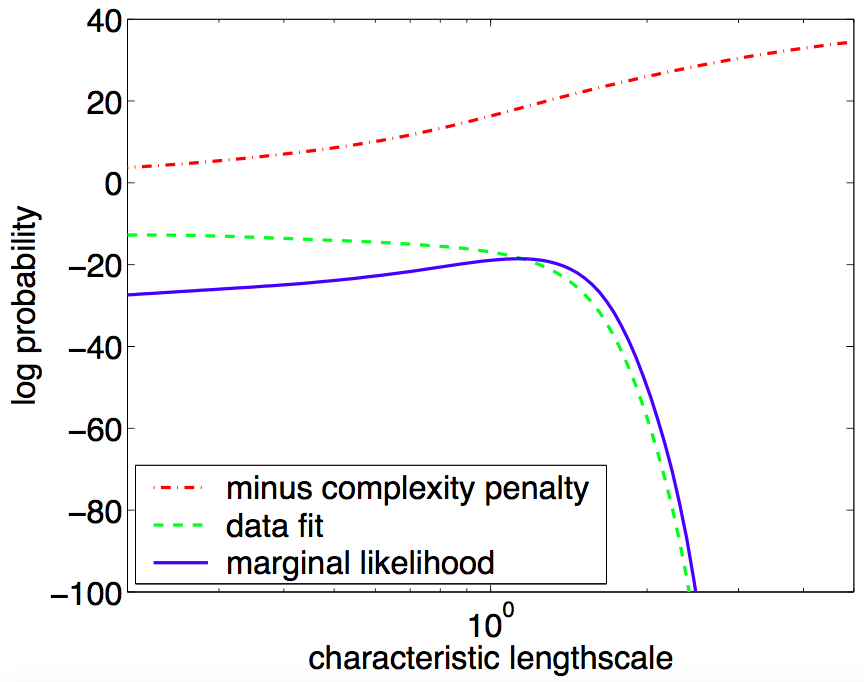
\includegraphics[width=0.5\linewidth]{loglikelihoodbreakdown.png}
\caption{ The log marginal likelihood function and the effect of its components\cite{rasmussen2006gaussian}  }
\end{figure}
\noindent 
To facilitate the optimisation, we can compute the gradients of the log marginal likelihood function with respect to hyperparameters, which has the form
	\begin{equation}
	\dfrac{\partial \log p( D \vert \boldsymbol{\theta}) }{\partial \theta_i} = \dfrac{1}{2} \mathbf{y}_n^T K_{\mathbf{y}}^{-1} \dfrac{\partial K_{\mathbf{y}}}{\partial \theta_i} K_{\mathbf{y}}^{-1}\mathbf{y}_n-\dfrac{1}{2} \mathrm{tr} \left (K_{\mathbf{y}}^{-1} \dfrac{\partial K_{\mathbf{y}}}{\partial \theta_i} \right ) = \dfrac{1}{2}\mathrm{tr} \left[ (\boldsymbol{\alpha} \boldsymbol{\alpha}^T- K_{\mathbf{y}}^{-1}) \dfrac{\partial K_{\mathbf{y}}}{\partial \theta_i} \right] 
	\end{equation} 
where $\boldsymbol\alpha=K_{\mathbf{y}}^{-1} \mathbf{y}_n$. Then, effective gradient-based optimisation algorithms such as conjugate gradients \cite{bishop2006pattern} can be employed to find the optimal set of hyperparameters. 
\\\\
However, the log marginal likelihood function is generally a non-convex function with multiple local optima \cite{bishop2006pattern}. Thus, maximum likelihood estimation may lead to hyperparameters corresponding to a bad local optimum, causing the problem of over-fitting. This is more likely to occur when the observation/training data set is small, which is the case for Bayesian optimisation, and the local optima of marginal likelihood are quite close \cite{rasmussen2006gaussian}.
\\\\ \noindent
If we have some prior knowledge about hyperparameters, we can combine the prior distribution over $\boldsymbol{\theta}$ with the marginal likelihood to implement the maximum a posteriori estimation. By Bayes rule, the posterior over the hyperparameters is 
\begin{equation} \label{hypposterior}
		p(\boldsymbol{\theta} \vert D_n ) = \frac{ p( D_n \vert \boldsymbol{\theta}) p( \boldsymbol{\theta} ) } {\int p( D_n \vert \boldsymbol{\theta}) p( \boldsymbol{\theta} ) d\boldsymbol{\theta} }
		\propto  p( D_n \vert \boldsymbol{\theta}) p( \boldsymbol{\theta} )
\end{equation} 
\begin{equation} \label{hypposterior}
		\Rightarrow \log p(\boldsymbol{\theta} \vert D_n) \propto  \log p( D_n \vert \boldsymbol{\theta}) + \log p( \boldsymbol{\theta} ).
\end{equation} 
Thus, maximising the log posterior over hyperparameters is equivalent to maximising the sum of the log marginal likelihood and the log prior. The maximum a posteriori estimation can be viewed as the maximum likelihood estimation with regulation, thus alleviating the problem of overfitting. 

\subsection{Marginalisation}
Both maximum likelihood estimation and maximum a posteriori estimation are not desirable as they give point estimates and ignore our uncertainty about the hyperparameters. In a fully Bayesian treatment of the hyperparameters, we should consider all possible hyperparameter values by marginalising the acquisition function (Equation \ref{acesbopa2}) with respect to the posterior  $p(\boldsymbol{\psi} \vert D_n )$ where $\boldsymbol{\psi}=\{\boldsymbol{\theta}, \eta\}$ :
 	 \begin{equation}
	 \alpha_{ESBOPA}(\mathbf{x} \vert D_n) = \int  \alpha_{ESBOPA}(\mathbf{x} \vert \boldsymbol{\Psi} , D_n ) p ( \boldsymbol{\Psi} \vert D_n) d\boldsymbol{\Psi}.
	 \end{equation}
Since complete marginalisation over hyperparameters is analytically intractable, the integral must be approximated using the Monte Carlo method \cite{hoffman2015} \cite{snoek2012practical}: 
	  \begin{equation}
\alpha_{ESBOPA}(\mathbf{x} \vert D_n) = H \Big[  \frac{1}{N} \sum_i^{N} p(y \vert D_n,\mathbf{x},\boldsymbol{\theta}^{(i)}, \eta^{(i)}) \Big] -  \frac{1}{2N} \sum_i^{N} \log \big[ 2\pi e \big(v_f(\mathbf{x} \vert D, \boldsymbol{\theta}^{(i)}, \eta^{(i)})+\sigma_n^2 \big) \big] 
   	  \end{equation}

\section{ESBOPA Algorithm}
The procedures of ESBOPA approach can be summarised by the following algorithm

\begin{algorithm}
\caption{ESBOPA Version2 }\label{ESBOPA }
\begin{algorithmic}[1]
\INPUT a test input $\mathbf{x}$; noisy observation data $D_n=\{(\mathbf{x}_{i},y_{i}) \vert i=1, \dots, n\}$
\Statex
	\State sample hyperparameters and $\eta$ : $\boldsymbol{\Psi}=\{\boldsymbol{\Theta}, \boldsymbol{\eta}\}= \{\boldsymbol{\theta}^{(j)},\eta^{(j)} \vert j=1, \dots, M\}$ from the posterior distribution $p(\boldsymbol{\psi} \vert D_n)$
	\For{j=1,$\dots, M$}
	\State use $f(\mathbf{x}) =\eta+\sfrac{1}{2}g(\mathbf{x})^2 $ to approximate $p(f \vert D_n,\mathbf{x},\boldsymbol{\theta}^{(j)}, \eta^{(j)})= \mathcal{GP} \big(m_f(\cdot),K_f(\cdot,\cdot)\big ) $
	
	3.1) compute $D_g=\{(\mathbf{x}_{i},g_{i}) \vert i=1, \dots, n\} $ where $g_{i}=\sqrt {2(y_{i}-\eta^{(j)})}$
	
	3.2) compute posterior distribution $ p(g \vert  D_g, \mathbf{x}, \boldsymbol{\theta}^{(j)},\eta^{(j)})=\mathcal{GP} \big (g; m_{g}(\cdot),K_{g}(\cdot,\cdot) \big)$
	
	3.3) approximate $p(f \vert D_n,\mathbf{x},\boldsymbol{\theta}^{(j)}, \eta^{(j)})$ using linearisation technique 
	
	\State compute $p(y \vert D_n,\mathbf{x},\boldsymbol{\theta}^{(j)}, \eta^{(j)}) =  \mathcal{GP} \big (m_f(\cdot),K_f(\cdot,\cdot)+ \sigma_n^2 \big)$
	
	\State compute $ H[p(y \vert D_n,\mathbf{x},\boldsymbol{\theta}^{(j)}, \eta^{(j)})] =0.5 \log \big[2\pi e \big (v_f(\mathbf{x} \vert D_n, \boldsymbol{\theta}^{(j)}, \eta^{(j)})+\sigma_n^2\big ) \big ] $
	
	\EndFor	
			
	\State estimate entropy of the gaussian mixture : 
	
	$ E1(\mathbf{x} \vert D_n) = H \Big[  \frac{1}{M} \sum_j^{M} p(y \vert D_n,\mathbf{x},\boldsymbol{\theta}^{(j)}, \eta^{(j)}) \Big] $
	
	\State compute the entropy expectation: $ E2(\mathbf{x} \vert D_n)= \frac{1}{2M} \sum_j^{M} \log \big[ 2\pi e \big(v_f(\mathbf{x} \vert D_n, \boldsymbol{\theta}^{(j)}, \eta^{(j)})+\sigma_n^2\big) \big] $ 	
	
	\State \textbf{return}  $\alpha_n(\mathbf{x} \vert D_n)=E1(\mathbf{x} \vert D_n)-E2(\mathbf{x} \vert D_n)$
	
\end{algorithmic}
\end{algorithm}
\noindent
Figure \ref{1DESBOPA} illustrates the sampling behaviour of ESBOPA method for a simple 1-D Bayesian optimisation problem. The optimisation process is started with three initial observation data. Subsequent query points are selected by maximising ESBOPA acquisition function which trades off exploitation and exploration. As more samples are taken, the mean of the posterior distribution for the objective function gradually resembles the objective function $f(\mathbf{x})$. The distribution for $\eta$ is set such that $\eta$ value is always lower than the minimum observation. As more information is gained, the distribution of $\eta$ converges to the global minimum $f(\mathbf{x}_*)$.
\\
\begin{figure} [p]
\label{1DESBOPA}
	\begin{subfigure}{.5\textwidth}
		  \centering
		  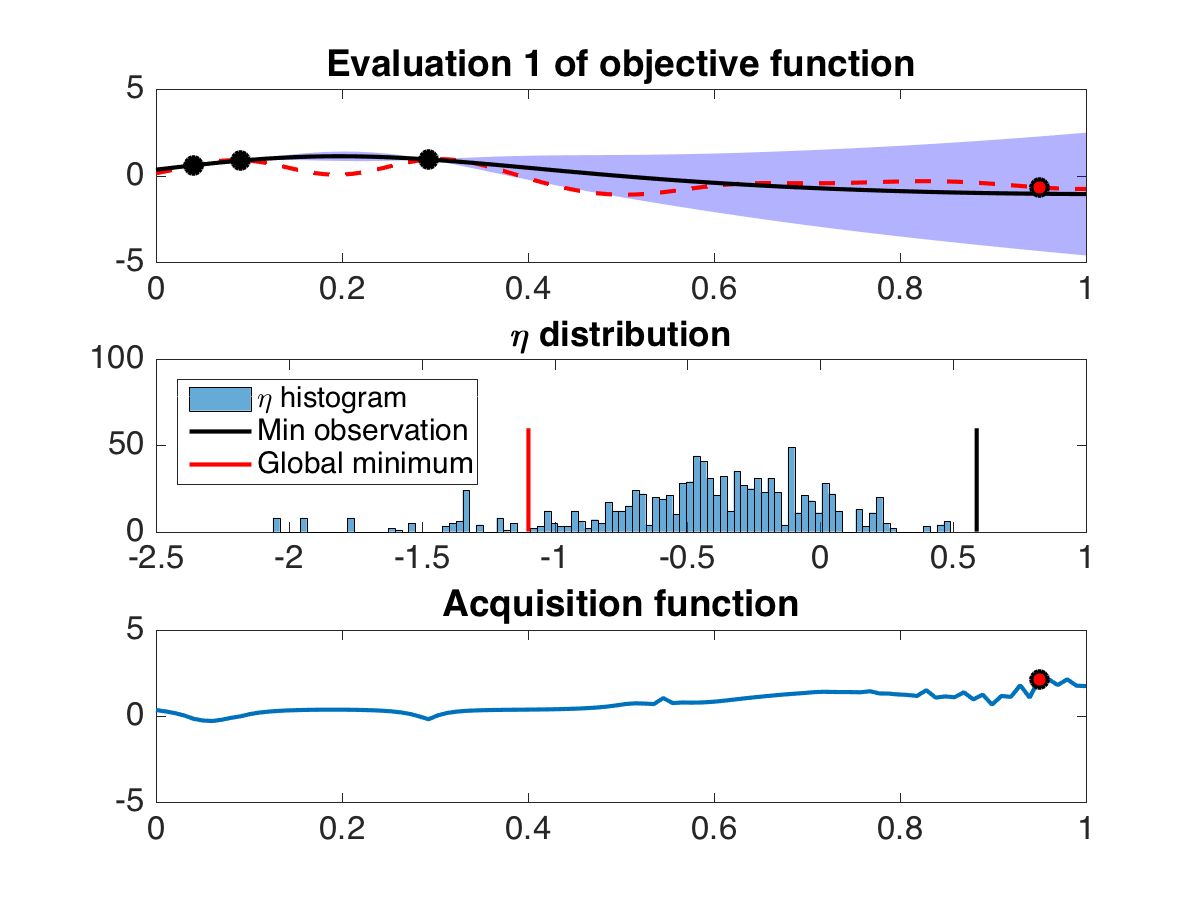
\includegraphics[width=1\linewidth]{ESBOPA_update_eta_prior_seed6_1.png}
 		% \caption{ evaluation=1}
 		% \label{fig:sfig1}
	\end{subfigure}
	\begin{subfigure}{.5\textwidth}
 		 \centering
 		 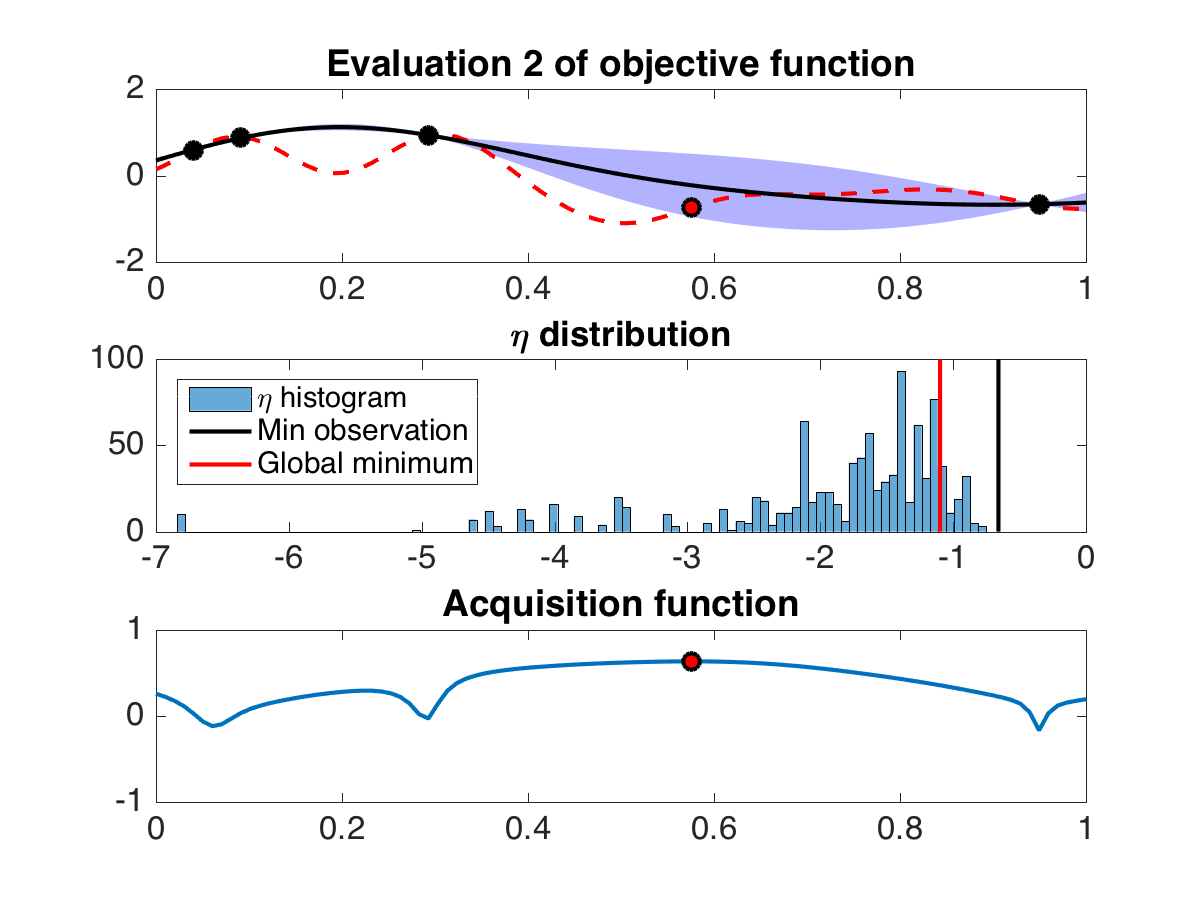
\includegraphics[width=1\linewidth]{ESBOPA_update_eta_prior_seed6_2.png}
  		%\caption{use parabolic approximation to draw $f^i$}
		%  \label{fig:sfig2}
	\end{subfigure}	
	\begin{subfigure}{.5\textwidth}
		  \centering
		  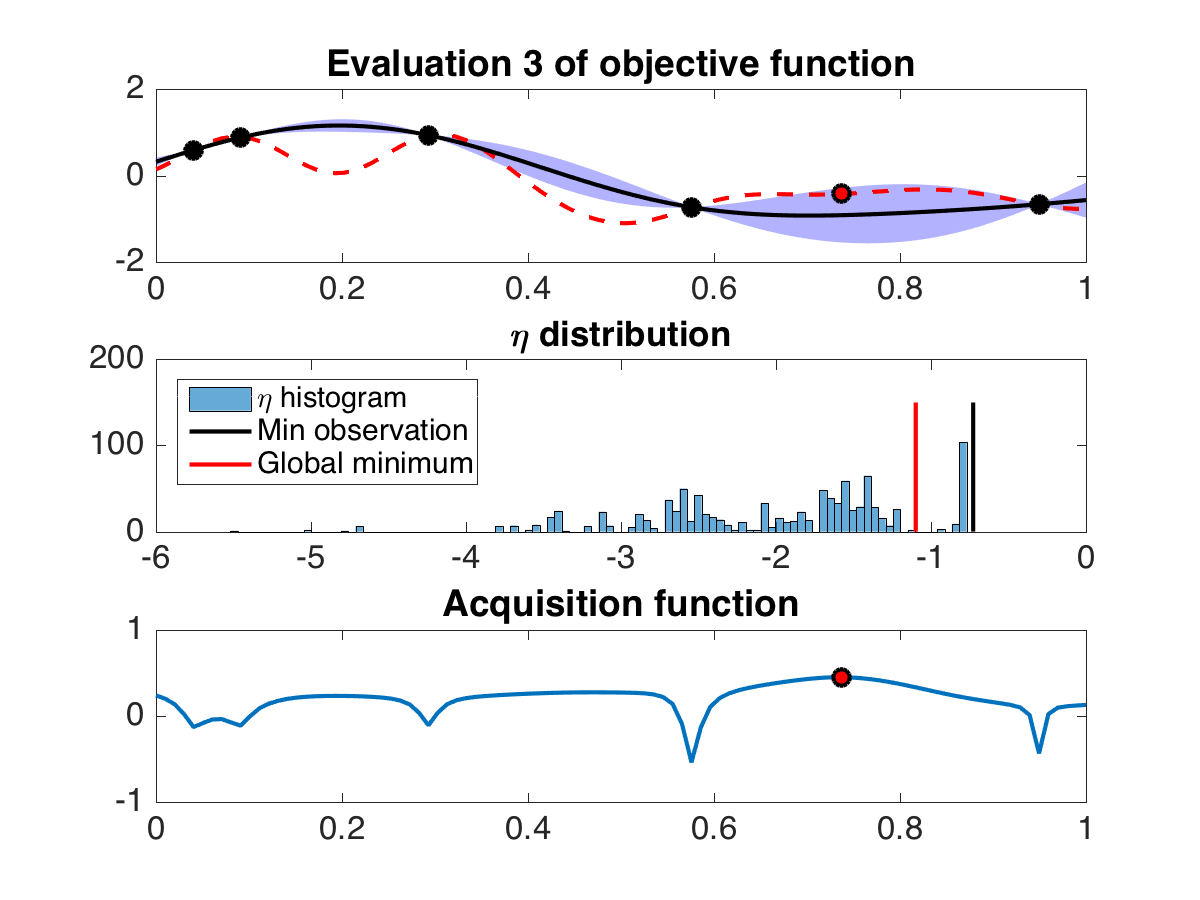
\includegraphics[width=1\linewidth]{ESBOPA_update_eta_prior_seed6_3.png}
 		% \caption{use posterior distribution to draw $f^i$}
 		% \label{fig:sfig1}
	\end{subfigure}
	\begin{subfigure}{.5\textwidth}
		  \centering
		  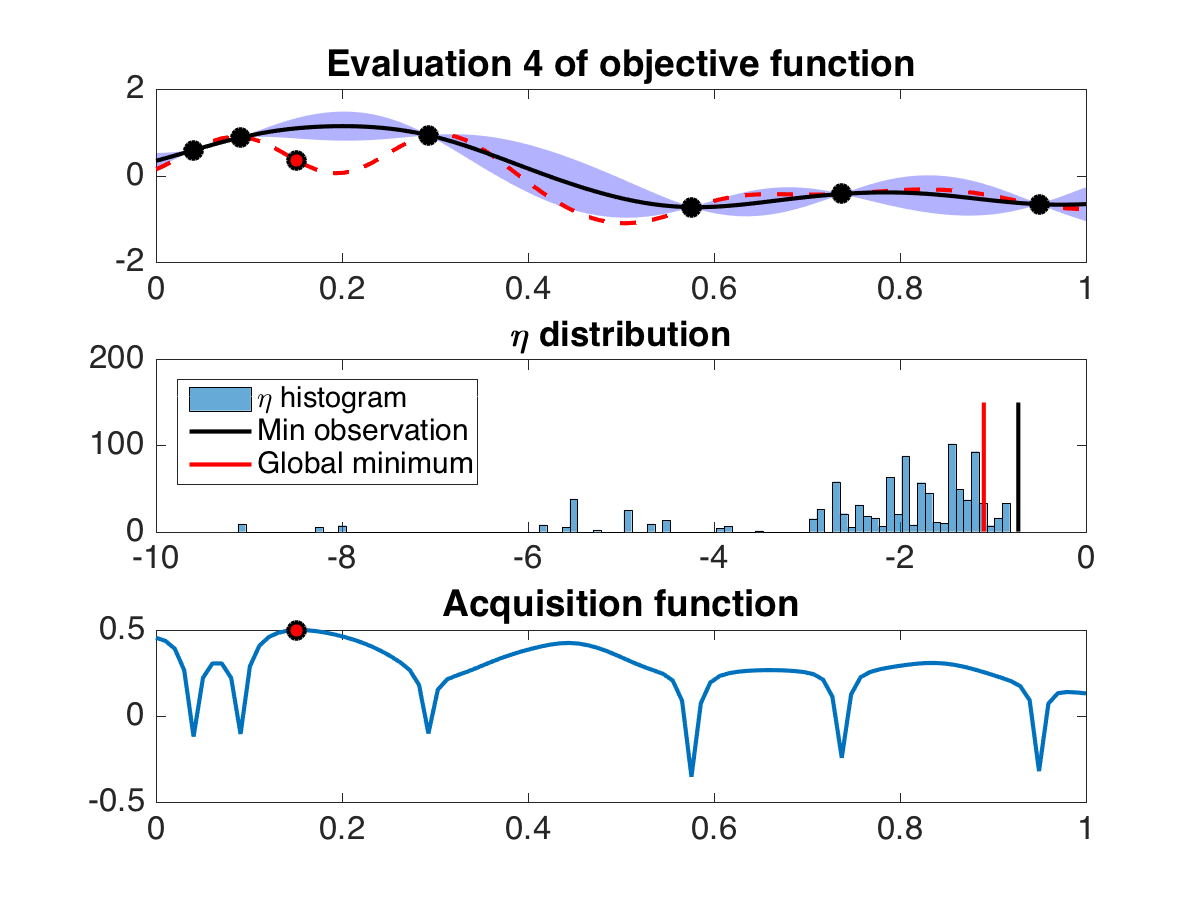
\includegraphics[width=1\linewidth]{ESBOPA_update_eta_prior_seed6_4.png}
 		% \caption{use posterior distribution to draw $f^i$}
 		% \label{fig:sfig1}
	\end{subfigure}
	\begin{subfigure}{.5\textwidth}
 		 \centering
 		 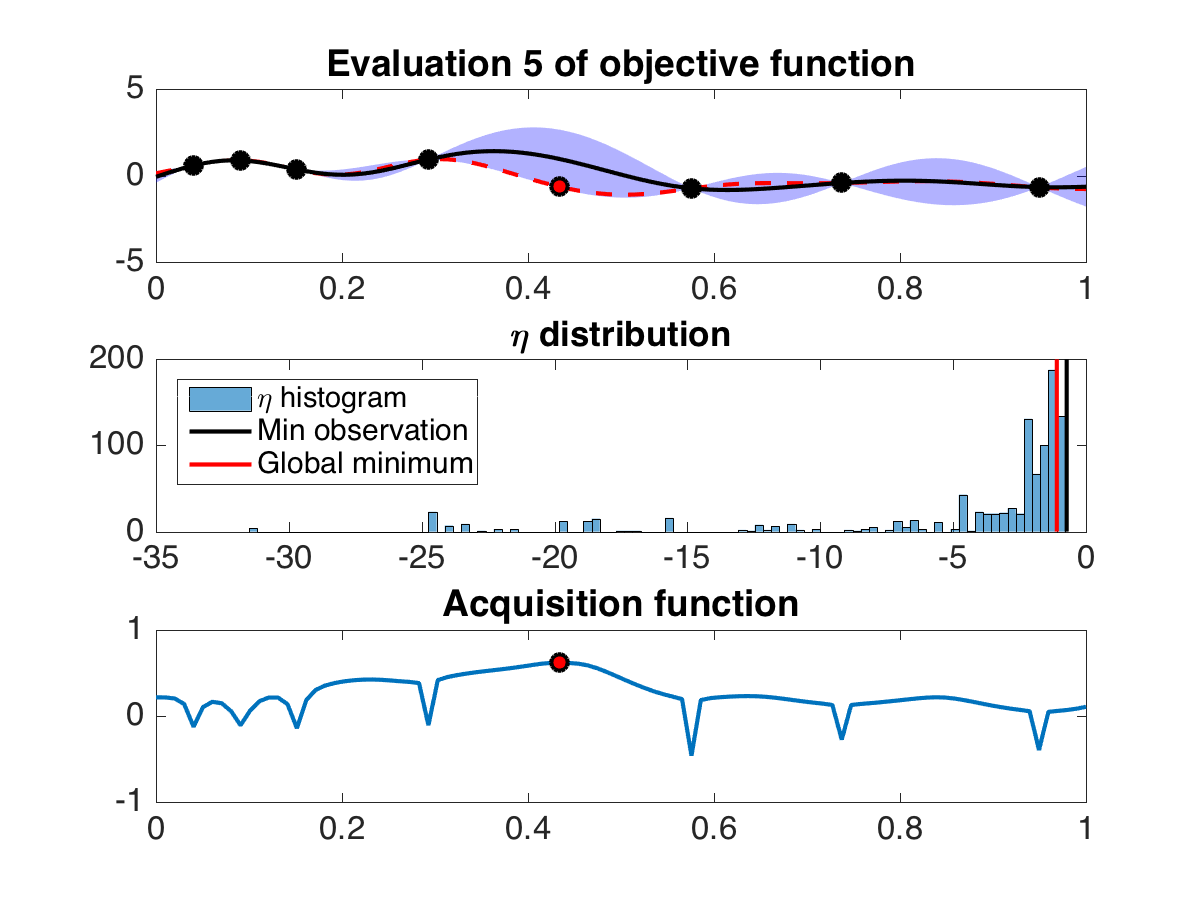
\includegraphics[width=1\linewidth]{ESBOPA_update_eta_prior_seed6_5.png}
  		%\caption{use parabolic approximation to draw $f^i$}
		%  \label{fig:sfig2}
	\end{subfigure}	
	\begin{subfigure}{.5\textwidth}
		  \centering
		  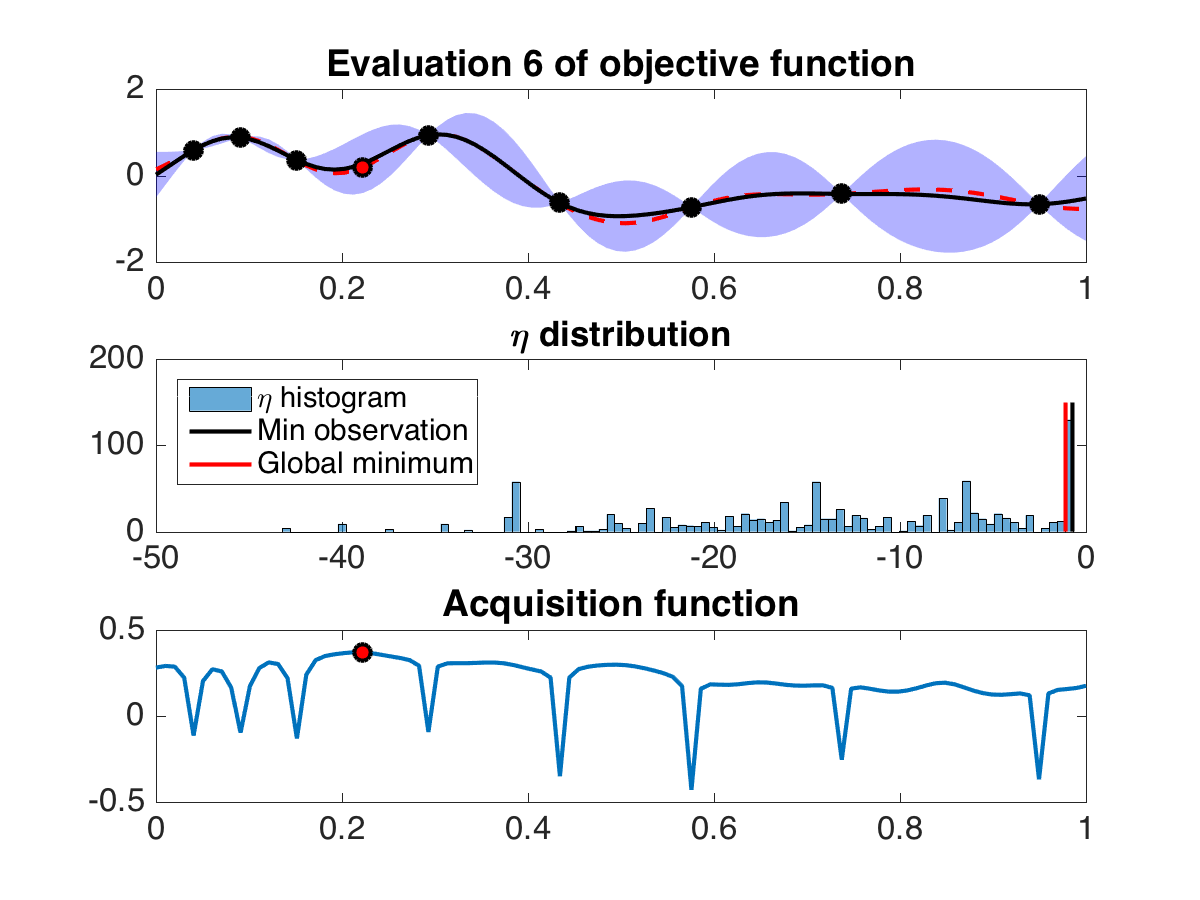
\includegraphics[width=1\linewidth]{ESBOPA_update_eta_prior_seed6_6.png}
 		% \caption{use posterior distribution to draw $f^i$}
 		% \label{fig:sfig1}
	\end{subfigure}
\caption{ Bayesian optimisation for a 1-D objective function using ESBOPA method. In each subfigure, the top plot shows the latent objective function (red dotted line), the posterior mean (black solid line) and the 95$\%$ confidence interval (blue shaded area) estimated by the Gaussian process model as well as the observation points (black solid dot) and the next query point (red solid dot with black edge).The middle plot is the histogram of $\eta$ samples and its relation to the minimum observation (black vertical line) and the true global minimum (red vertical line). The bottom plot illustrates ESBOPA acquisition function which is maximised to select the next query point.}
\end{figure}

%%  Approximations of the Entropy of a Gaussian Mixture Model %%
\section{Approximation of a Gaussian Mixture Entropy} \label{approxHGMM}

\subsection{Method 1: Taylor Expansion}

Huber et al. (2008) \cite{huber2008entropy}  propose a novel method for approximating the entropy of a Gaussian mixture model by using a Taylor-series expansion of the logarithm of the Gaussian mixture.
\\\\ \noindent
Let $ q (y)= \sum_i^{N} w_i  p(y \vert D_n,\mathbf{x},\eta^{(i)}) = \sum_i^{N} w_i  \mathcal{N}(y; m_i, \sigma_i^2)$. The Gaussians in the mixture are univariate in our case because the function value at a test location $\mathbf{x}$ is 1-D. The entropy of this mixture is: 
 	\begin{equation} \label{entropyofmixtureqh}
	H \left[ \frac{1}{N}  \sum_i^{N} p(y \vert D,\mathbf{x},\eta^{(i)}) \right] =H \left[ q(y) \right] = - \int q(y) \log h (y) \mathrm{d} y 
	\end {equation}
where $h(y)=q(y)$ but we uses different notations to differentiate the Gaussian mixture that's argument of the logarithm from that in front of the logarithm. 
\\\\
By expanding the logarithm term around the mean of each Gaussian term $m_i $ in $h(y)$, the resultant $R$-th order Taylor series is
	\begin{equation} \label{taylorexpoflogh}
	\log h (y) = \sum_{k=0} ^{R} \frac{(y - m_i)^k}{k !} \frac{\mathrm{d}^{k} \big(\log h(y) \big)} {\mathrm{d} y^k}\bigg \rvert_{y=m_i}.
	%=\sum_{k=0} ^{R} \frac{(y-m_i)^k}{k ! h( m_i)} \frac{ \mathrm{d}^{k} \big( h(y) \big)} {\mathrm{d} y^k}\bigg \rvert_{y= m _i}.
	\end {equation}
We then substitute equation \ref{taylorexpoflogh} into equation \ref{entropyofmixtureqh} and obtain
  	\begin{eqnarray*} 
	H \left[ q(y) \right] &=& - \int q(y) \log h (y) dy 
	\\&=& - \int \sum_i^{N} w_i  \mathcal{N}(y; m_i, \sigma_i^2) \log h (y) \mathrm{d} y
	\\&=& -  \sum_i^{N} w_i  \int  \mathcal{N}(y; m_i, \sigma_i^2) \sum_{k=0} ^{R} \frac{(y - m_i)^k}{k !} \frac{\mathrm{d}^{k} \big(\log h(y) \big)} {\mathrm{d} y^k}\bigg \rvert_{y=m_i}   \mathrm{d} y
	\\&=& -  \sum_i^{N} w_i  \sum_{k=0} ^{R} \frac{1}{k ! }  \frac{\mathrm{d}^{k} \big(\log h(y) \big)} {\mathrm{d} y^k}\bigg \rvert_{y=m_i}  \int  \mathcal{N}(y; m_i, \sigma_i^2) (y-m_i)^k \mathrm{d} y
	\end {eqnarray*}
where $ \int  \mathcal{N}(y; m_i, \sigma_i^2) (y-m_i)^k \mathrm{d} y$ is the $k$-th central moment of a Gaussian distribution and thus has a closed form. The $k$-th derivative of the logarithm of Gaussian mixture $h(y)$ can also be computed analytically because the derivatives of a Gaussian distribution always exist and Kronecker algebra can be used to achieve a compact representation \cite{huber2008entropy}. 
\\\\ \noindent
The entropy approximation by Taylor expansion faces the trade-off between the accuracy and computational burden as we can obtain more accurate approximations by including higher order Taylor-series terms at the expense of computational speed \cite{huber2008entropy}. Experiments with this approximation approach are carried out with a second-order Taylor-series expansion whose explicit form is provided by the Appendix in \cite{huber2008entropy}:
	\begin{equation}
	H \left[ \frac{1}{N}  \sum_{i=1}^{N} p(y \vert D_n,\mathbf{x},\eta^{(i)}) \right] \approx H_0[y] + H_2[y] 
	 =  - \sum_{i=1} ^N w_i \log h( m_i ) -  \sum_{i=1} ^N \frac{w_i \sigma_i^2}{2} F(m_i)
	\end{equation}
where $ F(y) = h(y)^{-1}\sum_{j=1}^N w_j \sigma_{j}^{-2} \left[ h(y)^{-1} (y - \mu_j) h' (y) + \sigma_j^{-2} (y- \mu_j)^2 -1 \right] \mathcal{N} (y; \mu_j,  \sigma_j^{2}) $.


\subsection{Method 2: Numerical Integration}

As mentioned before, one advantage of ESBOPA method is that it allows us to transform the entropy calculation from the multi-dimensional input space to the one-dimensional output space. This, thus, permits the use of numerical integration techniques to effectively compute the entropy of a Gaussian mixture.  %One advantage of using quadrature ??
Experiments with numerical integration are performed with the \textit{quad} function in MATLAB which utilises the adaptive Simpson quadrature. 

\subsection{Method 3: Simple Monte Carlo }

The first term in our ESBOPA acquisition function (Equation \ref{acesbopa2}) can be reformulated in the following way:
	\begin{eqnarray*}
	& & H \left[ \frac{1}{N}  \sum_i^{N} p(y \vert D_n,\mathbf{x},\eta^{(i)}) \right] 
	\\ &=& H \left[  \sum_i^{N} w_i  p(y \vert D_n,\mathbf{x},\eta^{(i)}) \right]   \hspace{0.5 cm} \text{  where  } \hspace{0.5cm}  w_i=  \frac{1}{N}
	\\ &=& - \int \left(  \sum_i^{N} w_i  p(y \vert D_n,\mathbf{x},\eta^{(i)})  \right) \log \left( \sum_i^{N} w_i  p(y \vert D_n,\mathbf{x},\eta^{(i)}) \right) \mathrm{d}y
	\\ &=& -  \sum_i^{N} w_i  \int p(y \vert D_n,\mathbf{x},\eta^{(i)})  \log \left( \sum_i^{N} w_i  p(y \vert D_n,\mathbf{x},\eta^{(i)}) \right) \mathrm{d}y	
	\end{eqnarray*}
By drawing $M$ samples of $y$ from $ p(y \vert D_n,\mathbf{x},\eta^{(i)}) $ and using Monte Carlo integration, the entropy of a Gaussian mixture can be approximated as  
	\begin{equation}
	 H \left[ \frac{1}{N}  \sum_i^{N} p(y \vert D_n,\mathbf{x},\eta^{(i)}) \right] \approx  -  \sum_i^{N} w_i  \left[ \frac{1}{M} \sum_j^{M} \log \left( \sum_i^{N} w_i  p(y^{(j)} \vert D_n,\mathbf{x},\eta^{(i)}) \right) \right]			
	\end{equation}
\\ \noindent
The accuracy of the simple Monte Carlo approximation  can be enhanced by increasing the sample size $M$. But larger number of samples will increase the computational burden. Thus, we also face a trade-off between the approximation precision and computational speed. 

\subsection{Experiments for Comparing Approximation Methods}
The following experiments are conducted to validate as well as compare the three entropy approximation  methods: 1) Huber's method that uses Taylor series expansion (Huber), 2) numerical integration that uses adaptive Simpson quadrature (Quadra) and 3) the simple Monte Carlo integration (MC). The approximation performance is assessed in terms of accuracy and computational speed. The optimal approximation method is then chosen based on the trade-off between the accuracy and computational demand. 
\\\\
The methodology of the tests can be summarised as follows: 
\begin{enumerate} [label={[\arabic*]}]
          \item Generate a Gaussian mixture as a weighted sum of N 1-D random Gaussian distributions
          \item For the Gaussian mixture, estimate its true entropy by using simple Monte Carlo method with large sample size (e.g. MC50000 )
          \item Use the 3 approximation methods to approximate the entropy of the Gaussian mixture. For the MC method, try it with different sample sizes  (e.g. MC10,MC100,MC1000)
          \item Compute and record the running time as well as absolute and fractional approximation errors for each method.
          \item Repeat the above processes for M different gaussian mixtures and compute the median running time and the median of the approximation errors. 
\end{enumerate} 
\noindent
With reference to Figure \ref{fig:fig_medi_abs_err} and \ref{fig:fig_medi_frac_err}, in the case of a single Gaussian($N=1$) distribution, there is a closed-form expression for its entropy. The Huber's method gives the exact true entropy solution, thus having 0 approximation error. The other 2 approximation methods (Quadra and MC) are compared against the true entropy value. It is evident that the approximation by Monte Carlo with 50000 samples (MC50000) is very close to the true value, which justifies our use of the approximation results of MC50000 as our yardstick for the cases of more than one Gaussians in the mixture. 
\\
\begin{figure} [H]
\label{fig:fig_medi_abs_err}
	\centering
	 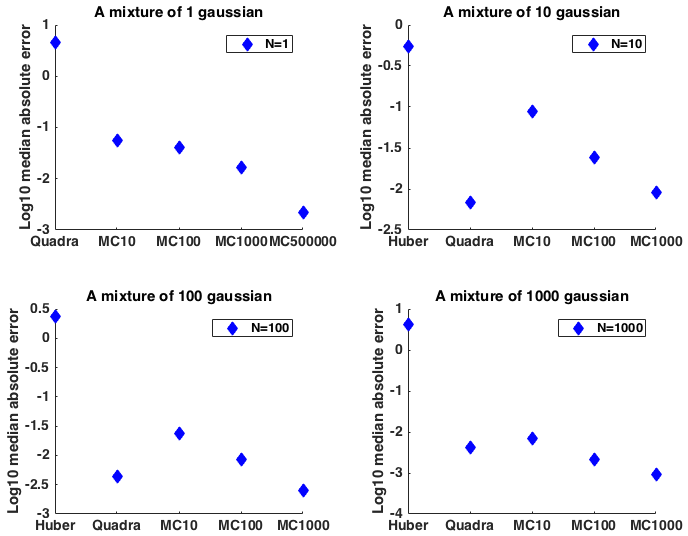
\includegraphics[width=0.7\linewidth]{Log_median_absolute_error.png}
 		% \label{fig:sfig1}
\caption{ Log median absolute error in approximating the entropy of a Gaussian mixture.}
\end{figure}

\begin{figure} [H]
\label{fig:fig_medi_frac_err}
	\centering
 	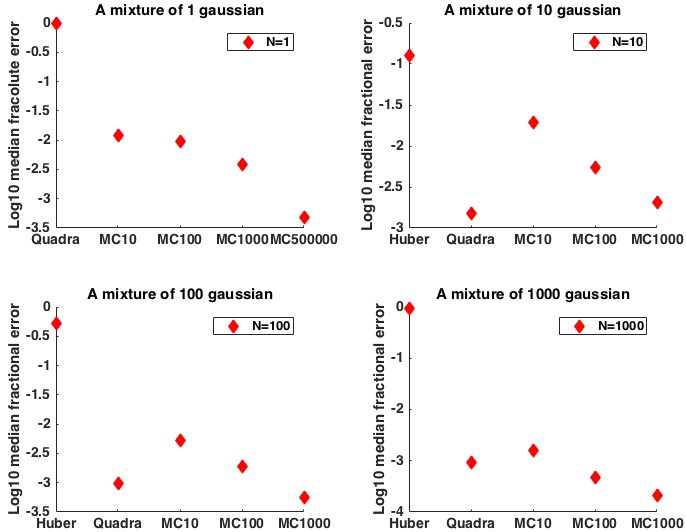
\includegraphics[width=0.7\linewidth]{Log_median_frac_error.png}
 		% \caption{use posterior distribution to draw $f^i$}
 		% \label{fig:sfig1}
\caption{ Log median fractional error in approximating the entropy of a gaussian mixture }
\end{figure}

\noindent
For a mixture of more than one Gaussian distribution ($N>1$),  the performances of all 3 approximation methods (Huber, Quadra, MC) are compared against the entropy value estimated by MC50000. The results in Figure  \ref{fig:fig_medi_abs_err} and \ref{fig:fig_medi_frac_err} show that Monte Carlo with a sample size of 1000 (MC1000) produces the most accurate approximation in terms of absolute and fractional approximation errors.  MC100 and quadrature (Quadra) also have relatively accurate approximation with low absolute and fractional error. The Huber method leads to the highest approximation errors. This may be due to the low order (order of 2) of Taylor-series expansion used in our experiments.  
\\\\
In Figure \ref{runningtime}, the running times of all 3 approximation methods are compared. As expected, the results show that the computation time increases as the number of Gaussians in the mixture rises. This is mainly due to the computation burden associated with the construction of the Gaussian mixture. More importantly, the quadrature method (Quadra) gains speed advantage as the number of gaussians in the mixture increases because the computational cost of approximation using quadrature does not increase with the number of Gaussian components in the mixture. The speed advantage of the quadrature method becomes more salient as we have more Gaussians in the mixture which is reflected in the growing difference among the running times of these methods. Since the number of gaussians in the mixture (N) is determined by the number of hyperparameter samples we use for  marginalisation in our algorithm, if we want to use a larger number of hyperparameter sets, we should adopt the quadrature method for fast approximation of the Gaussian mixture entropy at decent accuracy. 
\\
\begin{figure} [H]
\label{runningtime} 
\captionsetup{justification=centering}
	\centering
	 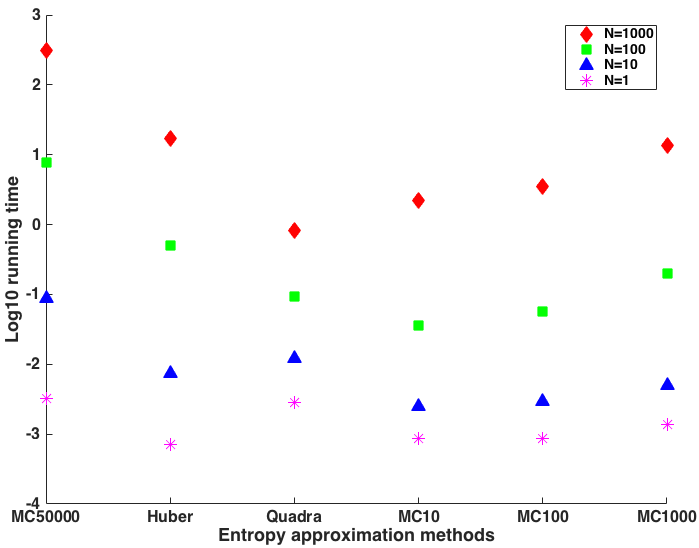
\includegraphics[width=0.7\linewidth]{Running_time.png}
 		% \caption{use posterior distribution to draw $f^i$}
 		% \label{fig:sfig1}
\caption{ Compare the running times of the approximation methods. }
\end{figure}

%%%%%%%%%%%%%%%%%%%%%%%%%%%%%%%%%%%%%%%%%%%%%%%%%
%%%%%%%%%%%%%%  Experiments  %%%%%%%%%%%%%%%%%%%%%%%%%
%%%%%%%%%%%%%%%%%%%%%%%%%%%%%%%%%%%%%%%%%%%%%%%%%

\chapter{Experiments and Results}
In this chapter, we will implement ESBOPA approach described above and compare its performance with some of the existing acquisition functions introduced in Section \ref{acqusitionfunction}. The first set of experiments are within model whereby ESBOPA methods will be tested using 1D and 2D test functions generated from a predetermined Gaussian process model. The second set of experiments will then evaluate ESBOPA algorithm with well-known benchmark test functions such as Branin-Hoo (2D), Rosenbrock(2D) as well as  Hartmann-6 (6D). 
\\\\
In all experiments, we use Metropolis Hastings algorithm \cite{bishop2006pattern} to sample hyperparameters $\boldsymbol{\theta}$ and $\eta$ and then marginalise all acquisition functions over the hyperparameters and $\eta$. The samples of hyperparameters and $\eta$ must fulfilll two conditions: 1) hyperparameters such as the characteristic length scale, output scale need to be positive and 2) $\eta$ is not greater than the minimum observation $y_{min}$. In order to enforce these two conditions, we assume the prior distributions of $ \log \boldsymbol{\theta}$ and $\eta - y_{min}$ are broad Gaussian distributions. We then generate $M$ samples of $ \{ \log \boldsymbol{\theta}^{(j)}, \eta^{(j)} - y_{min} \vert j=1, \dots, M \} $, from which the samples of $\{\boldsymbol{\theta}^{(j)}, \eta^{(j)} \vert j=1, \dots, M \}$ are reconstructed. 
\\\\
The posterior distribution $p(\boldsymbol{\Psi} \vert D_n)$, where $\boldsymbol{\Psi}=\{ \boldsymbol{\theta}, \eta \}$, is an essential element for the sampling process. We assume hyperparameters and $\eta$ are all independent and obtain the following expression by Bayes rule: 
 \[ p(\boldsymbol{\Psi} \vert D_n) \propto p( D \vert \boldsymbol{\Psi} ) p (\boldsymbol{\theta}) p(\eta) \]
 where 
 \[ p (\boldsymbol{\theta}) = \left \lvert \frac{ \mathrm{d} \log \boldsymbol{\theta}} { \mathrm{d} \boldsymbol{\theta}} \right \rvert p( \log \boldsymbol{\theta})= \frac{1} {\boldsymbol{\theta}} p( \log \boldsymbol{\theta}) ,\]
 \[ p(\eta) = p(y_{min}- \eta) = \left \lvert \frac{\mathrm{d} \log (y_{min}- \eta)} {\mathrm{d} \eta} \right \rvert p \big( \log (y_{min}- \eta) \big) =  \frac{1} { (y_{min}- \eta)} p \big( \log (y_{min}- \eta) \big) . \]
\noindent
Therefore, the logarithm of the unnormalised posterior distribution $\log \tilde p(\boldsymbol{\Psi} \vert D_n) $, from which we draw samples of hyperparameters and $\eta$, has the form: 
 \[ \log \tilde p(\boldsymbol{\Psi} \vert D_n) = \log p( D_n \vert \boldsymbol{\Psi} ) + \log p (\boldsymbol{\theta}) + \log p(\eta) \]
 where 
\[ \log p( D_n \vert \boldsymbol{\Psi} ) = -\frac{1}{2} \mathbf{y}_n^T [K_{f} (\mathbf{X}_n,\mathbf{X}_n') + \sigma_{n}^2 \mathbf{I} ]^{-1} \mathbf{y}_n - \frac{1}{2} \log \vert  K_{f} (\mathbf{X}_n,\mathbf{X}_n') + \sigma_{n}^2 \mathbf{I}\vert - \frac{n}{2} \log 2\pi,  \] 
 \[ \log p (\boldsymbol{\theta}) = \log \left[ \frac{1} {\boldsymbol{\theta}} p( \log \boldsymbol{\theta}) \right ] = \log p( \log \boldsymbol{\theta}) - \log \boldsymbol{\theta} , \]
 \[ \log p(\eta) = \log \left [ \frac{1} { (y_{min}- \eta)} p \big( \log (y_{min}- \eta) \big) \right ] = \log p \big( \log (y_{min}- \eta) \big) - \log (y_{min}- \eta)  . \]
\\
\noindent
In addition to hyperparameter sampling, we uses two common metrics to evaluate the performance of various Bayesian optimisation algorithms in all experiments \cite{hennig2012entropy}. The first metric is Immediate regret (IR) which is defined as:
\begin{equation} \label {IR}
IR=\vert f(\mathbf{x}_{*})- f(\hat{\mathbf{x}}_n)\vert 
\end{equation}
where $\mathbf{x}_{*}$ is the location of true global minimiser and $\hat{\mathbf{x}}_n$ is the location recommended by a Bayesian optimiser after $n$ iterations, which corresponds to the global minimiser of the posterior mean\cite{hernandez2014predictive}. The second metric is the Euclidean distance of an optimiser's best recommendation $\hat{\mathbf{x}}_n$ from true global minimiser $\mathbf{x}_{*}$, which is defined as
\begin{equation} \label{Euclidean}
\| L\| _{2} =\| \mathbf{x}_{*} - \hat{\mathbf{x}}_{n} \| . 
\end{equation} 

\section{Within-Model Comparison}
We first carried out within-model experiments over 1D and 2D unit domains (i.e $\mathcal{X} =[0, 1]$ and $\mathcal{X} =[0, 1] ^2$). The methodology of these experiments is similar to those adopted in \cite{hernandez2014predictive} \cite{hennig2012entropy} and is summarised below:
\begin{enumerate} [label={[\arabic*]}]
           \item Each test function is generated by sampling $m$ function values from the Gaussian process prior with a squared-exponential covariance function. The hyperparmeter values, namely length scale $ l$, output variance $\gamma^2 $ and noise variance $\sigma_n^2$ are specified by us. 
          \item  $M$ test functions are generated from the resulting Gaussian process posterior mean.
          \item  Evaluate the test function using three optimisation algorithms (PI,EI, ESBOPA) by MC sampling hyperparameter values. All the methods are initialized with three random measurements collected using latin hypercube sampling \cite{brochu2010tutorial}. 
          \item  After each iteration, each algorithm returns the global minimiser of the posterior mean over the test function $\hat{\mathbf{x}}_{n} $ as the best recommendation of the true minimiser $\mathbf{x}_{*}$. Evaluate the best recommendation for the minimum of the test function $f(\hat{\mathbf{x}}_{n})$. 
          \item Compute the immediate regret $IR = \vert f(\mathbf{x}_{*})- f(\hat{\mathbf{x}}_n)\vert $ and the Euclidean distance $ \| L\| _{2} = \| \mathbf{x}_{*} - \hat{\mathbf{x}}_{n} \| $. Repeat the above procedures for all $M$ test functions and plot the median of the $IR$ against the number of iterations. Confidence bands equal to one standard deviation are obtained using the bootstrap method. 
\end{enumerate} 
\noindent
Lobato et al. \cite{hernandez2014predictive} carried out within model experiments by fixing hyperparamters to the predetermined values  but in our within model experiments, we treat hyperparameters as unknown, which is more realistic, and marginalise over them during optimisation.   
% stop here %
\subsection{1D Test Functions}
This experiment is conducted over 50 different 1D test functions which are randomly generated using the procedures described above. Specifically, 50 samples of function values are used ($m$=50) and the hyperparmeters adopted for the GP prior are  $ l_1^2=0.01$, $\gamma^2=1 $,  $\sigma_n^2= 10^{-6}$. Figure \ref{1Dtestfunctions} shows six examples of the synthetic test functions. It is evident that almost all test functions generated via the within model approach are multimodal. Three optimisation algorithms are used, namely ESBOPA, EI and PI and the optimisation of each test function starts from 1 initial observation data. 
\\
\begin{figure} [H] \label{1Dtestfunctions}
	\centering
	 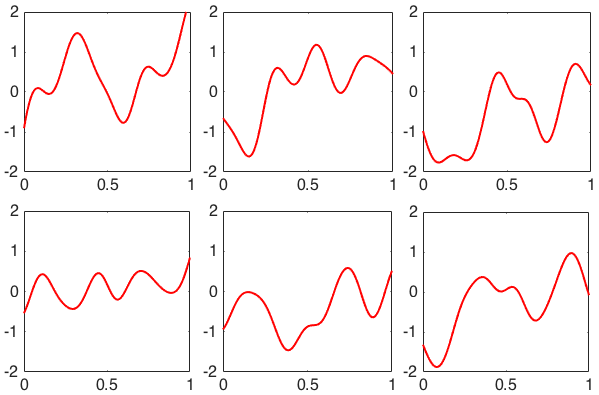
\includegraphics[width=0.8\linewidth]{1Dtestfunctions.png}
\caption{ Examples of 1D within model test functions. All  test function is constructed using a GP prior with a squared-exponential covariance function. The hyperparmeters of the GP model are  $ l_1^2=0.01$ , $\gamma^2=1 $,  $\sigma_n^2= 10^{-6}$} 
\end{figure}

\noindent
Figure \ref{1DtestIR} and Figure \ref{1DtestXnorm2} illustrate the resultant immediate regret and the Euclidean distance for all three algorithms starting from the first evaluation. For both evaluation metrics, ESBOPA beats PI throughout all 50 consecutive evaluations. ESBOPA initially loses out to EI but is able to catch up after 20 iterations. This may be due to PI is more exploitation-oriented than EI and thus tends to be trapped at local minimum during the initial iterations. All three algorithms converge to a similar constant level of accuracy eventually because the test functions are relatively simple. 
\\
\begin{figure} [H]
\label{1DtestIR}
	\centering
	 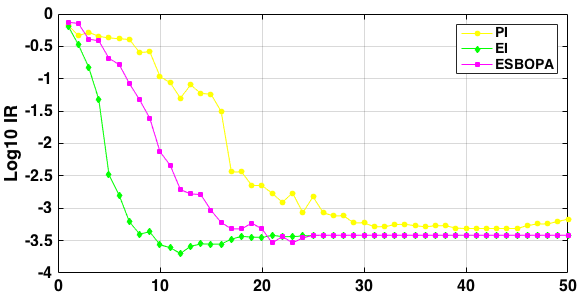
\includegraphics[width=0.8\linewidth]{1D_ESBOPAV4_IR.png}
 		% \label{fig:sfig1}
\caption{ Median immediate regrets of ESBOPA, EI and PI in the 1D within model experiments over 50 test functions.}
\end{figure}

\begin{figure} [H]
\label{1DtestXnorm2}
	\centering
	 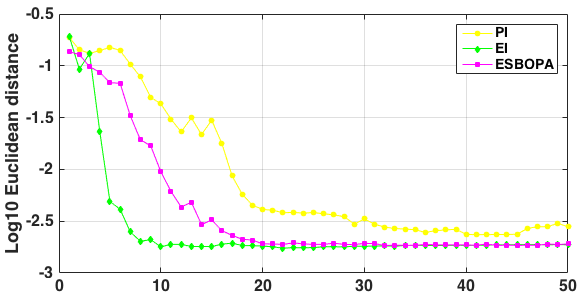
\includegraphics[width=0.8\linewidth]{1D_ESBOPAV4_Xnorm.png}
 		% \label{fig:sfig1}
\caption{ Median Euclidean distance between the global minimiser $\mathbf{x}_{*}$ and the best recommendation $ \hat{\mathbf{x}}_{n}$ of ESBOPA, EI and PI in the 1D within model experiments over 50 test functions}
\end{figure}
 \newpage
\subsection{2D Test Functions}
Similar to the 1D case, this experiment is carried out over 60 within model 2D test functions. These test functions are generated by sampling 50 function values ($m$=50)and setting the hyperparmeters of the GP prior to  $ l_1^2=l_2^2=0.1$ , $\gamma^2=1 $,  $\sigma_n^2= 10^{-6}$. Figure \ref{2Dtestfunctions} shows three examples of such 2D test functions. The optimisation processes for all algorithms start from 3 initial observation data.
\\
 \begin{figure} [H] \label{2Dtestfunctions}
	\centering
	 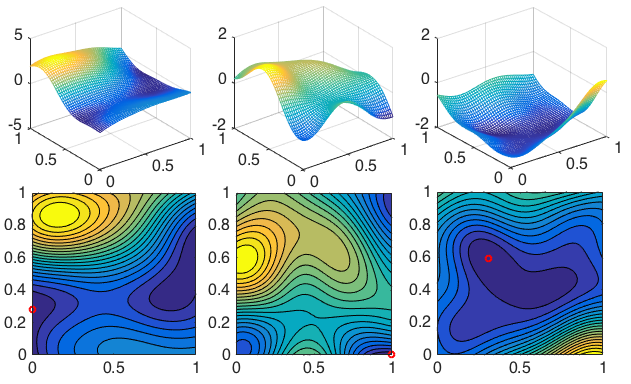
\includegraphics[width=0.9\linewidth]{2Dtestfunction.png}
\caption{Examples of 2D within model test functions which are generated using a GP prior with a squared-exponential covariance function. The hyperparmeters of the GP model are  $ l_1^2=l_2^2=0.1$ , $\gamma^2=1 $,  $\sigma_n^2= 10^{-6}$. Subfigures in the top row are the 3D mesh plots of the three test functions while their corresponding contour plots are shown in the bottom row.The location of the true global minimiser for each test function is indicated with a red circle.}
\end{figure}

\noindent
The median performance for all three algorithms over all test functions are displayed in Figure \ref{2DtestIR} and Figure \ref{2DtestXnorm2}. From the graphs, the ESBOPA method beats PI consistently but only gains an advantage over EI after taking enough number of iterations (over 40 iterations). One possible explanation for this initial poor performance of ESBOPA is that EI has comparatively more exploitative searching behaviours while ESBOPA requires more evaluations to gain information about the minimiser at the initial stage. More importantly, despite the quick convergence rate of EI, its searching accuracy stops at order of $IR \approx10^{-3}$ and $\| L\| _{2} \approx 10^{-2}$ after around 20 iterations. On the other hand, although ESBOPA converges at a slower rate, its accuracy keeps decreasing even after  45 iterations which is a promising sign that ESBOPA method could give more accurate results at the expense of convergence speed. 
\\
\begin{figure} [H] \label{2DtestIR}
	\centering
	 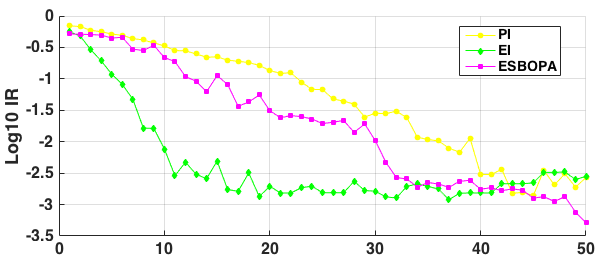
\includegraphics[width=0.8\linewidth]{2DtestESBOPAV3_seed_20_80IR.png}
\caption{ Median immediate regrets of ESBOPA, EI and PI in the within model experiments over 2D domain.}
\end{figure}

\begin{figure} [H]
\label{2DtestXnorm2}
	\centering
	 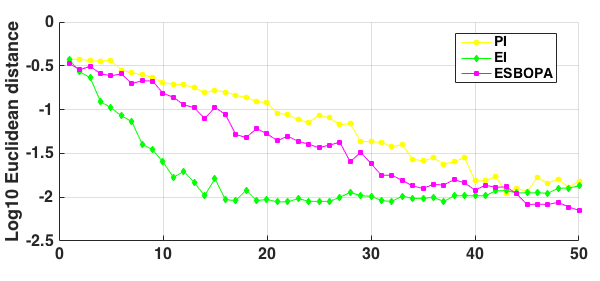
\includegraphics[width=0.8\linewidth]{2DtestESBOPAV3_seed_20_80Xnorm2.png}
\caption{ Median Euclidean distance between the global minimiser $\mathbf{x}_{*}$ and the best recommendation $ \hat{\mathbf{x}}_{n}$ of ESBOPA, EI and PI in the within model experiments over 2D domain.}
\end{figure}

\newpage
\section{Benchmark Test Functions}
In this section, we conduct another set of experiments using more challenging test functions such as Branin 2D, Rosenbrock 2D and Hartmann 6D. In all tests, the observation noise are set to a relatively low level $\sigma_n^2 = 10^{-3}$. 

\subsection{Branin 2D}
We use a modified version of the Branin 2D function which has the form: 
\begin{equation}
% a=15 x_1  - 5 ;
% b=15x_2;
	f(\mathbf{x}) = \frac{1}{10} \left[ \left ( \tilde x_2 - \frac{5.1} {4 \pi^2} \tilde x_1^2+\frac{5}{\pi} \tilde x_1 - 6 \right)^2 +10 \left(1-\frac{1}{8\pi} \right) \cos( \tilde x_1)+10 \right ] -15
\end{equation}
where $\tilde x_1=15 x_1 -5$ and $\tilde x_2=15 x_2 $.
\\\\
The modified Branin function has exactly the same shape and minimiser locations as the original Branin function as shown in Figure \ref{2DBranin}. However, its output range changes from [ 0.3979, 308.1291] to [-14.9602, 15.8129] and its input scale changes from $ x_1 \in [-5,10] , x_2 \in [0, 15] $ to $ x_1,x_2 \in [0,1] $.  The global minimum of the modified Branin 2D function is  -14.9602 at $\mathbf{x}_{*} = [0.1239, 0.8183],  [0.5428, 0.1517]$ and $ [0.9617,0.1650]$. 
\\
\begin{figure} [H]
\label{2DBranin}
	\centering
	 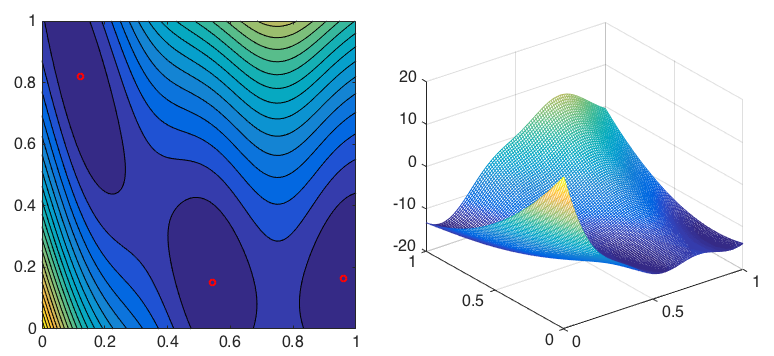
\includegraphics[width=0.9\linewidth]{Branin2D.png}
\caption{ The modified Branin 2D function with the globally minimum value of -0.9973 at three locations $\mathbf{x}_{*} = [0.1239, 0.8183],  [0.5428, 0.1517]$ and $ [0.9617,0.1650]$, denoted by red circles.}
\end{figure}

\noindent
The experiments with the Branin 2D function start from three initial observations. The performance of ESBOPA approach is compared with those of PI and EI in Figure \ref{2DBraninIR} and Figure \ref{2DBraninXnorm2}.  Similar to the case for the 2D within model experiments, ESBOPA experiences a slow convergence rate, thus losing out to EI and PI at the initial stage. However,  as more evaluations are taken, the performance of both improvement-based methods start to stabilise while the optimisation error of ESBOPA continues to decrease. This enables ESBOPA to catch up EI and PI and surpass them slightly in the end. 
\\
\begin{figure} [H] \label{2DBraninIR}
	\centering
	 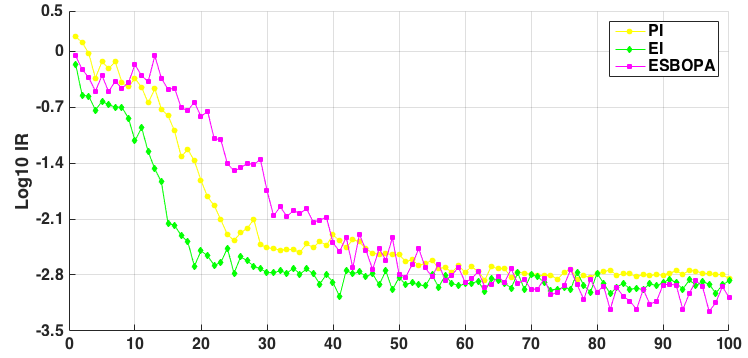
\includegraphics[width=0.8\linewidth]{2DBranin_ESBOPA_V4IR.png}
\caption{ Median immediate regrets of ESBOPA, EI and PI in the Branin 2D problem.}
\end{figure}

\begin{figure} [H]
\label{2DBraninXnorm2}
	\centering
	 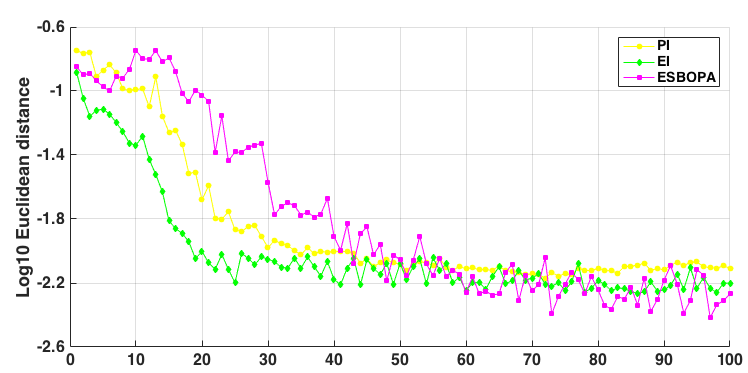
\includegraphics[width=0.8\linewidth]{2DBranin_ESBOPA_V4Xnorm2.png}
\caption{ Median Euclidean distance between the global minimiser $\mathbf{x}_{*}$ and the best recommendation $ \hat{\mathbf{x}}_{n}$ of ESBOPA, EI and PI in the Branin 2D problem.}
\end{figure}
\noindent
One interesting point we would like to illustrate through the Branin problem is the fundamentally different mechanisms behind ESBOPA and improvement-based approaches. As shown in Figure \ref{2Dbraninevaluationpoints}, the locations for evaluation proposed by ESBOPA spread across the whole domain but those by EI and PI tend to quickly concentrate at the zones of low functional values. Yet, ESBOPA is still able to predict the location of the global minimimum from such scattered evaluation samples. This different querying behaviour is due to the fact that information-based approaches such as ESBOPA aim to select the query point that maximises the information gain about the minimiser but improvement-based approaches such as EI and PI choose the query point that leads to an improvement over the current best function value observed \cite{shahriari2016taking}. 
\\
\begin{figure} [H] \label{2Dbraninevaluationpoints}
	\centering
	 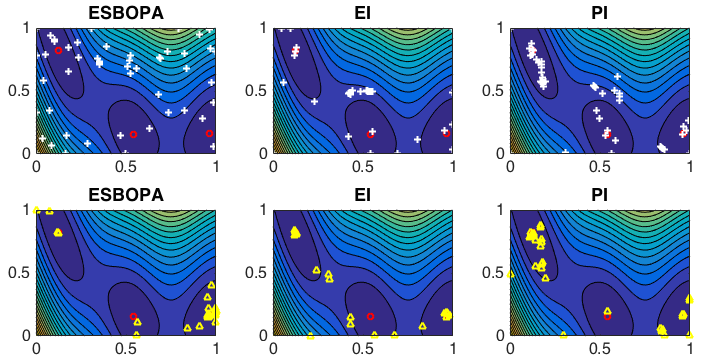
\includegraphics[width=1.0\linewidth]{Branin_evaluataions.png}
\caption{ 50 evaluations taken by ESBOPA, EI and PI in the Branin 2D problem. In the top row row of subfigures, the white crosses indicate the consecutive 50 evaluation samples proposed by the three algorithms. In the bottom row of subfigures, the yellow triangles indicate the 50 best guesses of the global minimiser recommended by all three algorithms after each corresponding evaluation.}
\end{figure}


\subsection{Rosenbrock 2D}
The Rosenbrock 2D function, also known as Rosenbrock's banana function, contains its global minimum inside a long narrow valley, which makes optimisation difficult. In our experiments, we modified the function to have an input scale of $ [-1,1]^2 $ and an output range of $[-10, 9]$ . The modified Rosenbrock 2D function preserves the valley shape as shown in Figure \ref{} and has the form:
\begin{equation}
f(\mathbf{x}) = a (1- \tilde x_1 )^2 + b ( \tilde x_2 - \tilde x_1^2) ^2 - c
\end{equation}
where $\tilde x_1 = 2 x_1$, $\tilde x_2 = 2 x_2$, $a=\sfrac{1}{200}$, $b=\sfrac{1}{2}$, $c=10$. The global minimum of the modified Rosenbrock 2D function is  -10 at $\mathbf{x}_*=[0.5, 0.5]$. 
\\
\begin{figure} [H]
\label{2Drosenbrock}
	\centering
	 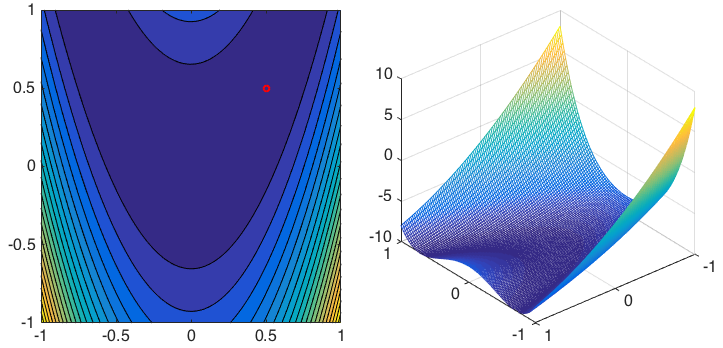
\includegraphics[width=0.9\linewidth]{rosenbrock2D.png}
\caption{The modified Rosenbrock 2D function with the globally minimum value of -10 at $\mathbf{x}_*=[0.5, 0.5]$, denoted by the red circle.}
\end{figure}
\noindent
As shown in Figure \ref{Rosenbrock_ESBOPAV4_IR}, ESBOPA outperforms EI and PI after 30 evaluations and then stays better than the other two approaches in searching the minimum off the Rosenbrock function. The advantage of ESBOPA over EI and PI is more obvious in predicting the location of the global minimiser $\mathbf{x}_{*}$ as shown in Figure \ref{Rosenbrock_ESBOPAV4_Xnorm}. In this case, although the greedy improvement-based approaches can quickly identify the parabolic flat valley in the problem, entropy-based approach does a better job in searching the global minimum in the valley where function values are very close.
\\
\begin{figure} [H] \label{Rosenbrock_ESBOPAV4_IR}
	\centering
	 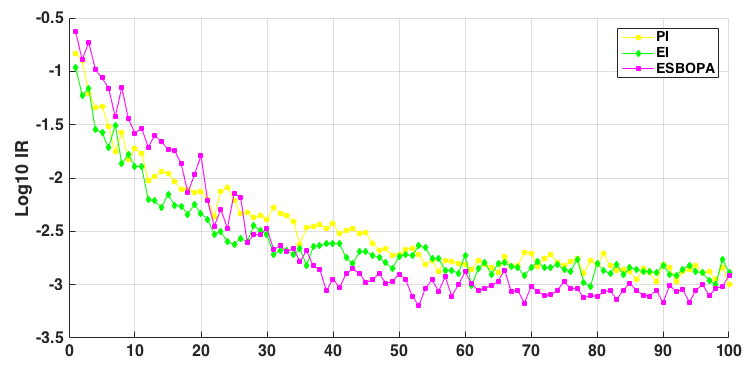
\includegraphics[width=0.8\linewidth]{Rosenbrock_ESBOPAV4_IR.png}
\caption{ Median immediate regrets of ESBOPA, EI and PI in the Rosenbrock 2D problem.}
\end{figure}

\begin{figure} [H]
\label{Rosenbrock_ESBOPAV4_Xnorm}
	\centering
	 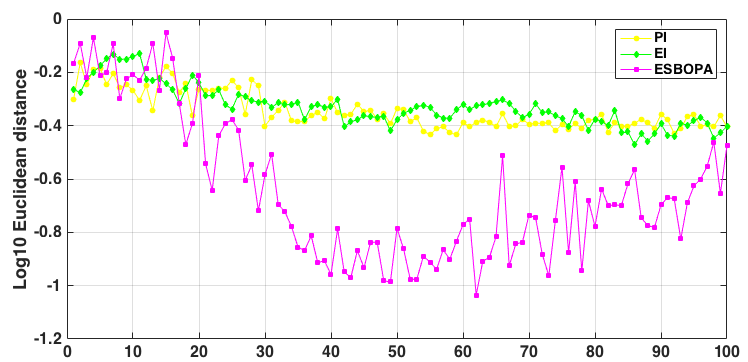
\includegraphics[width=0.8\linewidth]{Rosenbrock_ESBOPAV4_Xnorm.png}
\caption{ Median Euclidean distance between the global minimiser $\mathbf{x}_{*}$ and the best recommendation $ \hat{\mathbf{x}}_{n}$ of ESBOPA, EI and PI in the Rosenbrock 2D problem.}
\end{figure}

\subsection{Hartmann 6D}
To further generalise our tests, we apply these algorithms to an even higher dimensional problem - Hartmann 6-D function (defined in $[0,1] ^6 $). The modified formula of Hartmann 6D has the following form: 
\begin{equation}
f(\mathbf{x}) = 1.5 - \sum_{i=1}^{4} \alpha_i \exp \left [ - \sum_{j=1}^6 A_{ij} ( x_j - P_{ij}) ^2 \right] , \hspace{12pt}\text{with}
\end{equation}
\[ \alpha = [ 1.0, 1.2, 3.0, 3.2 ] ^T\] 
\[ \bold{A} = \begin{bmatrix} 
	10    &	3	&	17	&	3.5	&	1.7	&	8	\\
    	0.05 &	10 	&	17	& 	0.1	&	8	&	14	\\
	3	&	3.5	&	1.7	&	10	&	17	&	8	\\
	17	&	8	&	0.05	&	10	&	0.1	&	14
\end{bmatrix}
\]
\[ \bold{P} = \begin{bmatrix} 
	0.1312	&	0.1696	&	0.5569	&	0.0124	&	0.8283	&	0.5886\\
         0.2329	&	0.4135	&	 0.8307	&	0.3736	&	0.1004	&	0.9991\\
         0.2348	&	0.1451	&	0.3522	&	0.2883	&	0.3047	&	0.6650\\
         0.4047	&	0.8828	&	0.8732	&	0.5743	&	0.1091	&	0.0381\\
\end{bmatrix}.
\]
where $x_i \in [0,1]$ for all $i=1, \dots , 6$. Thus, the Hartmann 6-D function has a global minimum of -1.8224 at $\mathbf{x}_* = [0.20169, 0.150011, 0.476874, 0.275332, 0.311652, 0.6573]$
\\\\
The tests start from 9 initial observations because of the higher dimension of the Hartmann function used. The optimisation performances of ESBOPA, EI and PI are presented in Figure \ref{6DHartIR} and \ref{6DHartXnorm}. In terms of immediate regrets, PI demonstrates the best performance followed by EI. ESBOPA has an initial advantage over EI but is overtaken by EI after around 60 iteration. 
Similar results are observed in \cite{hernandez2014predictive} as PES delivers consistently worse performance than EI in the Hartmann 6D functions. One explanation for the relatively poor performance of ESBOPA and PES in this problem is that information-theoretic approaches take more iterations to explore in high dimensional space, enabling the more greedy improvement-based approaches to gain advantage in optimising the relatively simple Hartmann function \cite{hernandez2014predictive}. 
\\\\
However, in the input space (Figure \ref{6DHartXnorm}), the best guess by ESBOPA is consistently closer to the true minimiser in terms of Euclidean distance than that predicted by EI. ESBOPA also perform better than PI before 60 evaluations in searching the minimiser location. 
\\
\begin{figure} [H] \label{6DHartIR}
	\centering
	 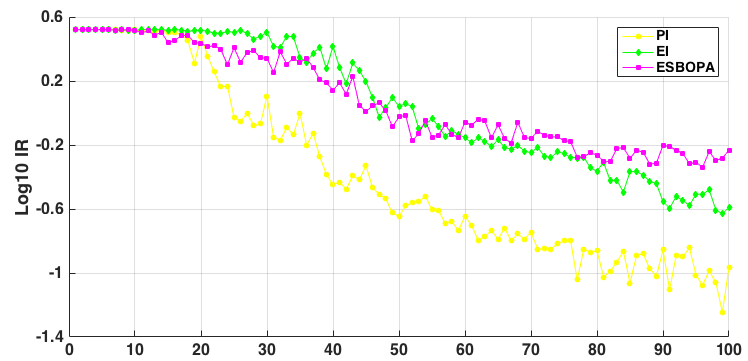
\includegraphics[width=0.8\linewidth]{Hartmann6D_ESBOPAV4_IR.png}
\caption{ Median immediate regrets for ESBOPA, EI and PI in the experiments with Hartmann 6D.}
\end{figure}

\begin{figure} [H]
\label{6DHartXnorm}
	\centering
	 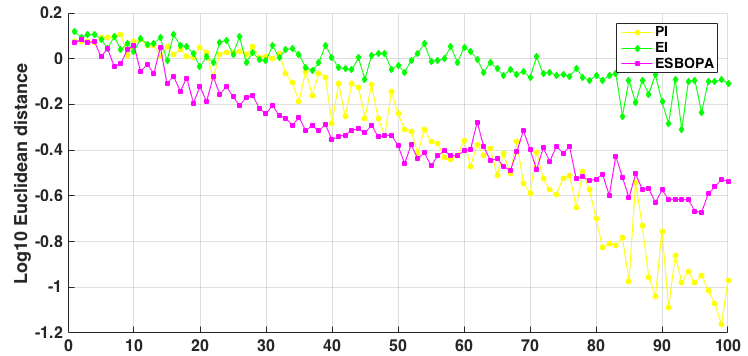
\includegraphics[width=0.8\linewidth]{Hartmann6D_ESBOPAV4_1_X_norm.png}
\caption{ Median Euclidean distance between the global minimiser $\mathbf{x}_{*}$ and the best recommendation $ \hat{\mathbf{x}}_{n}$ for ESBOPA, EI and PI in the experiments with Hartmann 6D.}
\end{figure}

\section{The Effect of Noise on Performance}
In the above experiments, the measurement noise level is set to a negligibly low level of $\sigma^2=10^{-3}$ or $10^{-6}$. However, in real world, the observation noise might be non-trivial and a good optimisation algorithm should be able to find the global minimiser even in the presence of relatively high noise level. Therefore, in this section, we would test and compare the optimisation performance of different acquisition functions under the effect of different noise levels. 
\\\\
Figrue \ref{RosenbrocknoisyIRandL2} shows that the optimisation results of ESBOPA, EI and PI acquisition functions applied to the Rosenbrock 2D problem at different noise levels. As the variance of observation noise $\sigma_n^2$ increases from 0.001 to 0.1, ESBOPA is still able to accurately identify the unknown global minimiser $\mathbf{x}_*$ and its performance stays close to those of EI and PI. However, EI and PI seem to do slightly better job than ESBOPA under the effect of high noise level $\sigma_n^2= 10^{-1}$. This advantage of EI and PI under high observation noise is more evident in the case of the Branin 2D problem (Figure \ref{BraninnoisyIRandL2}). 
\\
%% figures for Rosenbrock
\begin{figure} [H]
\label{RosenbrocknoisyIRandL2}
	\begin{subfigure}{.5\textwidth}
		  \centering
		  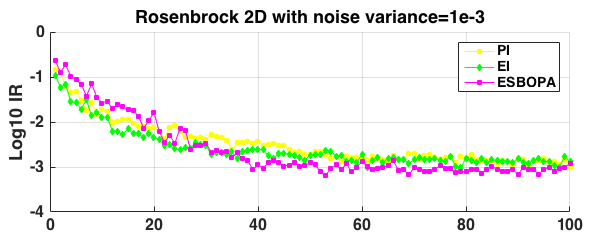
\includegraphics[width=1\linewidth]{Rosenbrock1e-3_ESBOPAV4_IR.png}
 		% \caption{ evaluation=1}
 		% \label{fig:sfig1}
	\end{subfigure}
	\begin{subfigure}{.5\textwidth}
 		 \centering
 		 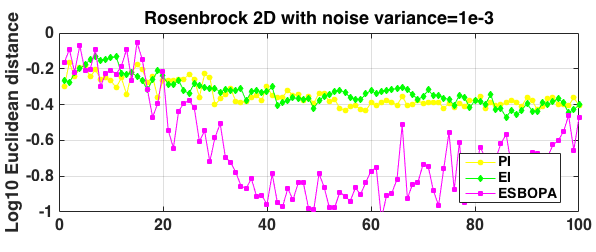
\includegraphics[width=1\linewidth]{Rosenbrock1e-3_ESBOPAV4_Xnorm.png}
  		%\caption{use parabolic approximation to draw $f^i$}
		%  \label{fig:sfig2}
	\end{subfigure}	
	\begin{subfigure}{.5\textwidth}
		  \centering
		  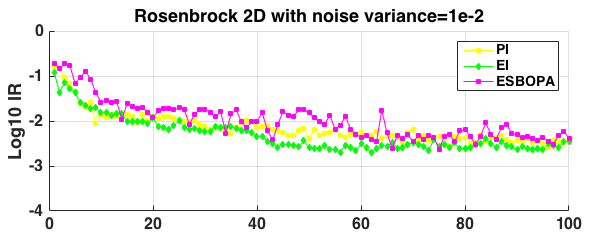
\includegraphics[width=1\linewidth]{Rosenbrock1e-2_ESBOPAV4_IR.png}
 		% \caption{use posterior distribution to draw $f^i$}
 		% \label{fig:sfig1}
	\end{subfigure}
	\begin{subfigure}{.5\textwidth}
		  \centering
		  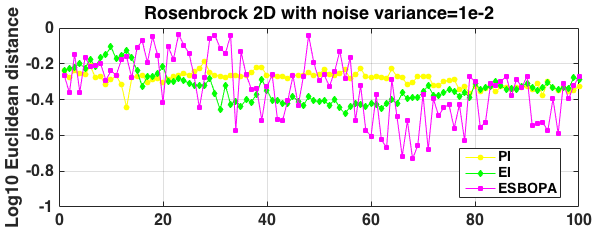
\includegraphics[width=1\linewidth]{Rosenbrock1e-2_ESBOPAV4_Xnorm.png}
 		% \caption{use posterior distribution to draw $f^i$}
 		% \label{fig:sfig1}
	\end{subfigure}
	\begin{subfigure}{.5\textwidth}
 		 \centering
 		 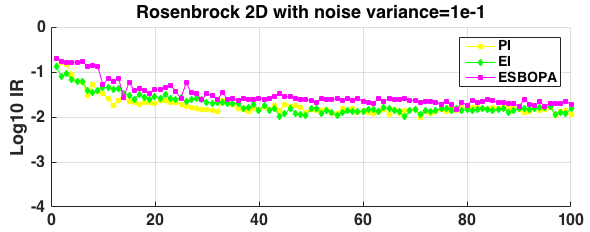
\includegraphics[width=1\linewidth]{Rosenbrock1e-1_ESBOPAV4_IR.png}
  		%\caption{use parabolic approximation to draw $f^i$}
		%  \label{fig:sfig2}
	\end{subfigure}	
	\begin{subfigure}{.5\textwidth}
		  \centering
		  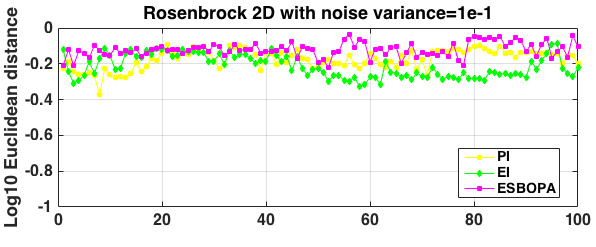
\includegraphics[width=1\linewidth]{Rosenbrock1e-1_ESBOPAV4_Xnorm.png}
 		% \caption{use posterior distribution to draw $f^i$}
 		% \label{fig:sfig1}
	\end{subfigure}
\caption{ Comparison of ESBOPA, EI and PI in the Rosenbrock 2D problem with noise levels 0.001, 0.01, 0.1. Subfigures on the left column show the results of the median immediate regret. Subfigures on the right column show the results of the median Euclidean distance between the global minimiser $\mathbf{x}_{*}$ and the best recommendation $ \hat{\mathbf{x}}_{n}$   regret.}
\end{figure}

\begin{figure} [H]
\label{BraninnoisyIRandL2}
	\begin{subfigure}{.5\textwidth}
		  \centering
		  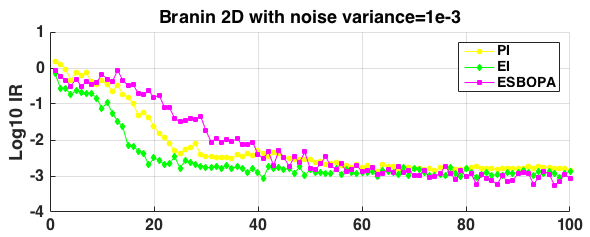
\includegraphics[width=1\linewidth]{Branin15noise1e-3_sigma100_ESBOPA_V4_IR.png}
 		% \caption{ evaluation=1}
 		% \label{fig:sfig1}
	\end{subfigure}
	\begin{subfigure}{.5\textwidth}
 		 \centering
 		 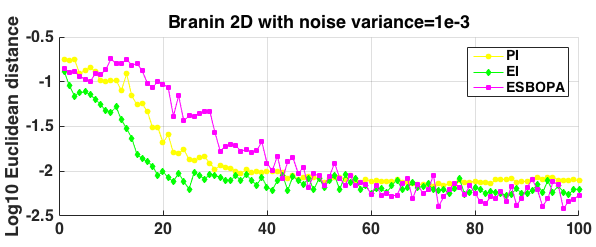
\includegraphics[width=1\linewidth]{Branin15noise1e-3_sigma100_ESBOPA_V4_Xnorm.png}
  		%\caption{use parabolic approximation to draw $f^i$}
		%  \label{fig:sfig2}
	\end{subfigure}	
	\begin{subfigure}{.5\textwidth}
		  \centering
		  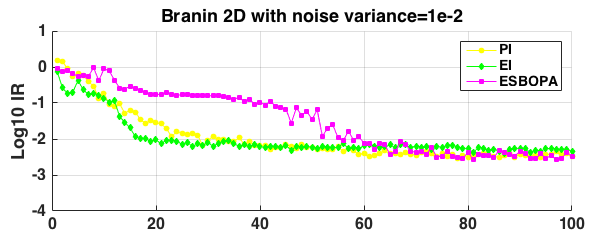
\includegraphics[width=1\linewidth]{Branin15noise1e-2_sigma100_ESBOPA_V4_IR.png}
 		% \caption{use posterior distribution to draw $f^i$}
 		% \label{fig:sfig1}
	\end{subfigure}
	\begin{subfigure}{.5\textwidth}
		  \centering
		  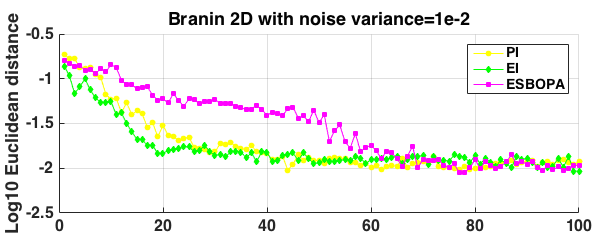
\includegraphics[width=1\linewidth]{Branin15noise1e-2_sigma100_ESBOPA_V4_Xnorm.png}
 		% \caption{use posterior distribution to draw $f^i$}
 		% \label{fig:sfig1}
	\end{subfigure}
	\begin{subfigure}{.5\textwidth}
 		 \centering
 		 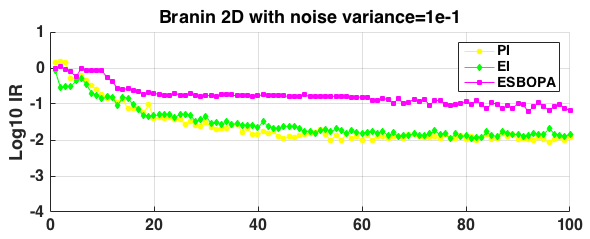
\includegraphics[width=1\linewidth]{Branin15noise1e-1_sigma100_ESBOPA_V4_IR.png}
  		%\caption{use parabolic approximation to draw $f^i$}
		%  \label{fig:sfig2}
	\end{subfigure}	
	\begin{subfigure}{.5\textwidth}
		  \centering
		  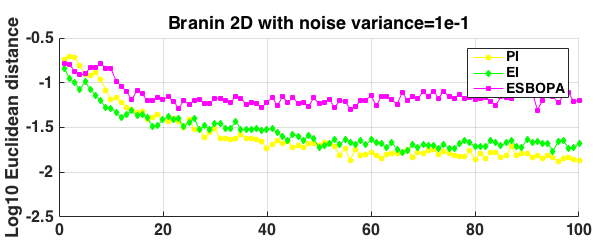
\includegraphics[width=1\linewidth]{Branin15noise1e-1_sigma100_ESBOPA_V4_Xnorm.png}
 		% \caption{use posterior distribution to draw $f^i$}
 		% \label{fig:sfig1}
	\end{subfigure}
\caption{ Comparison of ESBOPA, EI and PI in the Branin 2D problem with noise levels 0.001, 0.01, 0.1. Subfigures on the left column show the results of the median immediate regret. Subfigures on the right column show the results of the median Euclidean distance between the global minimiser $\mathbf{x}_{*}$ and the best recommendation $ \hat{\mathbf{x}}_{n}$   regret. }
\end{figure}

\chapter{Conclusion}
The project successfully develops a novel entropy based algorithm, called ESBOPA in short, for Bayesian optimisation. With the creative use of the parabolic approximation and the hyperparameter $\eta$, ESBOPA approach requires less sampling efforts and fewer approximations in its implementation as compared to existing information-theoretic approaches such as Entropy Search (ES) and Predictive Entropy Search (PES). Meanwhile, ESBOPA approach is also compatible with a wider range of covariance functions and enjoys the merit of working in the one-dimensional output space. Our ESBOPA method is tested via within model experiments and several challenging benchmark optimisation problems. On the whole, the results demonstrate a desirable and very promising optimisation performance in comparison with the two popular acquisition functions, Expected Improvement and Probability of Improvement. Therefore, ESBOPA method offers a very competitive alternative to the existing heuristics for Bayesian optimisation and our project makes a concrete contribution to the development of the information-based approaches. 
\\\\
Our research work can definitely be extended in the many areas. First, if given more time, we would test ESBOPA with more complex real world optimisation problems and compare ESBOPA with a wider range of current heuristics such as PES, ES and random search. Second, ESBOPA approach relies heavily on the prior distribution over $\eta$ which explicitly represent the global minimum. In our project, we just use a gaussian distribution for $\eta$ and set the hyperparameters defining the distribution ( i.e. mean and variance ) arbitrarily. However, another optimisation process can be applied to fine-tune the hyperparameters defining the $\eta$ distribution and other appropriate distributions such as gamma distribution are also worth exploring. With a more well-defined $\eta$ distribution, the performance of ESBOPA can be further enhanced. In addition, ESBOPA approach can also be improved by incorporating derivative observations at $\eta$. 

{\small\bibliographystyle{plain}
\addcontentsline{toc}{chapter}{Bibliography}
\bibliography {references}\clearpage}

\end{document}